% arara: manual

% Arara, the cool TeX automation tool
% Copyright (c) 2012 -- 2018, Paulo Roberto Massa Cereda
% All rights reserved.
%
% Redistribution and  use in source  and binary forms, with  or without
% modification, are  permitted provided  that the  following conditions
% are met:
%
% 1. Redistributions  of source  code must  retain the  above copyright
% notice, this list of conditions and the following disclaimer.
%
% 2. Redistributions in binary form  must reproduce the above copyright
% notice, this list  of conditions and the following  disclaimer in the
% documentation and/or other materials provided with the distribution.
%
% 3. Neither  the name  of the  project's author nor  the names  of its
% contributors may be used to  endorse or promote products derived from
% this software without specific prior written permission.
%
% THIS SOFTWARE IS  PROVIDED BY THE COPYRIGHT  HOLDERS AND CONTRIBUTORS
% "AS IS"  AND ANY  EXPRESS OR IMPLIED  WARRANTIES, INCLUDING,  BUT NOT
% LIMITED  TO, THE  IMPLIED WARRANTIES  OF MERCHANTABILITY  AND FITNESS
% FOR  A PARTICULAR  PURPOSE  ARE  DISCLAIMED. IN  NO  EVENT SHALL  THE
% COPYRIGHT HOLDER OR CONTRIBUTORS BE  LIABLE FOR ANY DIRECT, INDIRECT,
% INCIDENTAL, SPECIAL, EXEMPLARY,  OR CONSEQUENTIAL DAMAGES (INCLUDING,
% BUT  NOT LIMITED  TO, PROCUREMENT  OF SUBSTITUTE  GOODS OR  SERVICES;
% LOSS  OF USE,  DATA, OR  PROFITS; OR  BUSINESS INTERRUPTION)  HOWEVER
% CAUSED AND  ON ANY THEORY  OF LIABILITY, WHETHER IN  CONTRACT, STRICT
% LIABILITY, OR TORT (INCLUDING NEGLIGENCE OR OTHERWISE) ARISING IN ANY
% WAY  OUT  OF  THE USE  OF  THIS  SOFTWARE,  EVEN  IF ADVISED  OF  THE
% POSSIBILITY OF SUCH DAMAGE.
\documentclass[a4paper,oneside,12pt]{memoir}

\usepackage[T1]{fontenc}
\usepackage[utf8]{inputenc}
\usepackage[margin=2.5cm]{geometry}
\usepackage{arara}
\usepackage[record,postpunc=dot]{glossaries-extra}

\newcommand{\araraversion}{4.0}
\newcommand{\todo}[1]{\fbox{\em#1}}

\glssetcategoryattribute{abbreviation}{glossdesc}{firstuc}
\glssetcategoryattribute{general}{glossname}{firstuc}
\glssetcategoryattribute{general}{glossdesc}{firstuc}

\setabbreviationstyle{short-nolong-desc}
\renewcommand{\glsxtrshortdescname}{%
 \protect\glsabbrvfont{\the\glsshorttok} (\the\glslongtok)%
}

% No automated sorting. The list is just in order of definition.
% If the list gets too long, we can switch to using bib2gls.
 \newabbreviation
 [description={an interface that allows users to interact
through graphical components, such as buttons and menus}]
 {GUI}{GUI}{Graphical User Interface}

 \newabbreviation
 [description={an organisation that develops and promotes Internet standards}]
 {IETF}{IETF}{Internet Engineering Task Force}

 \newabbreviation
 [description={a virtual machine that enables Java programs to be run}]
 {JVM}{JVM}{Java Virtual Machine}

 \newabbreviation
 [description={a hybrid, dynamic, statically typed, embeddable
 expression language and runtime for the Java platform},
 location={(See Chapter~\ref{chap:mvel}.)}]
 {MVEL}{MVEL}{MVFLEX Expression Language}

\newglossaryentry{orb-tag}{name={orb tag},
 description={a dynamic element of an \gls{MVEL} template which is
 evaluated at runtime}}

\newabbreviation
 [description={a simple computer programming environment that takes
  a single expression (input), evaluates it and results the result}]
 {REPL}{REPL}{Read--Eval--Print Loop}

\newabbreviation
 [description={a database language}]
 {SQL}{SQL}{Structured Query Language}

\newabbreviation
 [description={a markup language that defines a set of rules for
encoding documents in a format that is both human-readable and
machine-readable}]
 {XML}{XML}{Extensible Markup Language}

\newabbreviation
 [description={human-friendly data, commonly used for configuration
files but also used for data storage or transmission},
 location={(See Chapter~\ref{chap:yaml}.)}]
 {YAML}{YAML}{YAML Ain't Markup Language}
 
\begin{document}

\begin{titlingpage}
\vspace*{2em}

\begin{center}

\includegraphics[scale=0.7]{../logos/logo2.pdf}

\vspace{4em}

\begin{tcolorbox}[
  boxrule=0pt,
  colback=araracolour,
  top=1em,
  bottom=1em
]
  \color{white}
  \centering
  \Huge
  \sffamily
  \bfseries User manual
\end{tcolorbox}

\vspace{6em}

{\large\em Paulo Cereda, Marco Daniel,\\
Brent Longborough, and Nicola Talbot\par}

\vspace{3em}

\href{mailto:cereda.paulo@gmail.com}{\fpemail{0.4}}%
\quad\href{https://github.com/cereda/arara}{\fpgithub{0.4}}%
\quad\href{http://twitter.com/paulocereda}{\fptwitter{0.4}}

\vfill

{\color{araracolour}
\LARGE
\sffamily
\bfseries
Version \araraversion}

\end{center}
\end{titlingpage}

\chapterstyle{araraheadings}
\pagestyle{headings}
\frontmatter
\nouppercaseheads

\cleardoublepage

\vspace*{25em}

\begin{flushright}
\em No birds were harmed in the making of this manual.
\end{flushright}

% !TeX root = ../arara-manual.tex
\chapter*{Foreword}
\label{chap:foreword}

\epigraph{That deserves no less than a ``Holy guacamole!''.}{\textsc{Gonzalo Medina}}

{\setlength{\parskip}{1em}
Creating a PDF from \LaTeX\ code can be quite tiresome. Suppose I am using \TeX works and I have a document that has a bibliography, glossary and index, then I need to select the \rbox{pdflatex} tool and click on the typeset button, then select the \rbox{bibtex} tool and click on the typeset button, then select the \rbox{makeindex} tool and click on the typeset button, then select the \rbox{makeglossaries} tool (which I may need to add first) and click on the typeset button, then select the \rbox{pdflatex} tool and click on the typeset button, and once more to ensure all the cross-references are up to date. Then I edit the document and have to go through that whole process all over again!

Automation makes life so much simpler. Instead of all those tools that I need to keep selecting, I just need one tool, in this case \arara, which will do all the necessary work for me behind the scenes.

Some automation tools try to be clever, but there are invariably exceptions that trip them up. \arara\ does not try to be clever; it just does what it is told to do. The instructions are provided as special comments in the source code that \TeX\ ignores, but they are human-readable and can also provide a hint to non-\arara\ co-authors as to what tools are required in order to complete the document build.

The new improved \arara\ version 4.0 now comes with some exciting features, such as the ability to use conditionals, and it definitely ranks as my favourite automation tool for document creation. Paulo has done a great job, and I would like to take this opportunity to thank
him for his patience in dealing with my many feature requests!}

\vfill

\begin{flushright}
Nicola Louise Cecilia Talbot\\
\emph{on behalf of the \arara\ team}
\end{flushright}

% !TeX root = ../arara-manual.tex
\chapter*{Prologue}
\label{chap:prologue}

\epigraph{Moral of the story: never read the
documentation, bad things happen.}{\textsc{David Carlisle}}

{\setlength{\parskip}{1em}
Writing software is easy. Writing \emph{good} software is extremely difficult. When the counter stopped at version 3.0, Brent, Marco and I decided it was time for \arara\ to graduate and finally be released in \TeX\ Live. My life had changed.

It was a success. A lot of people liked the idea of explicitly telling our tool how to compile their \TeX\ dcouments instead of relying on guesswork. It was indeed a cool concept! But then, the inevitable happened: a lot of bugs had emerged from the dark depths of my humble code.

In all seriousness, \emph{I was about to give up}. My code was not awful, but there were a couple of critical and blocking bugs. Something very drastic had to be done in order to put \arara\ back on track. Then, walking on faith, I decided to rewrite the tool entirely from scratch. In order to achieve this goal, I created a \href{https://github.com/cereda/nightingale}{sandbox} and started working on the new code.

It was my redemption. Nicola helped me with the new version, writing code, fixing bugs and suggesting new features. Soon, we all achieved a very pleasant result. It was like \arara\ was about to hatch again. Version 4.0 was definitely at our hands. Now, it is up to you.

Surprisingly, this humble user manual is not the best resource for learning about our tool. If you really want to see \arara\ in action, I strongly recommend \href{https://www.dickimaw-books.com/latex/admin}{\LaTeX\ for administrative work}, an amazing book freely available for download. The author is, of course, Nicola herself! She explains how \LaTeX\ can be used for administrative work, such as writing correspondence, performing repetitive tasks or typesetting problem sheets on exam papers. And \arara\ is there!

Enjoy the new version. Happy \TeX ing with \arara!
\par}

\vfill

\begin{flushright}
Paulo Roberto Massa Cereda\\
\emph{on behalf of the \arara\ team}
\end{flushright}

\chapter*{License}
\label{chap:license}

\epigraph{Anything that prevents you from being friendly, a good neighbour, is a terror tactic.}{\textsc{Richard Stallman}}

\arara\ is licensed under the \href{http://www.opensource.org/licenses/bsd-license.php}{New BSD License}. It is important to observe that the New BSD License has been verified as a GPL-compatible free software license by the \href{http://www.fsf.org/}{Free Software Foundation}, and has been vetted as an open source license by the \href{http://www.opensource.org/}{Open Source Initiative}.

\vfill

\begin{messagebox}{New BSD License}{araracolour}{\icinfo}{white}
\footnotesize

\includegraphics[scale=0.25]{../logos/logo1.pdf}

Copyright \textcopyright\ 2012--2018, Paulo Roberto Massa Cereda\\
All rights reserved.

\vspace{1em}

Redistribution and use in source and binary forms, with or without modification, are permitted provided that the following conditions are met:

\begin{itemize}
\item Redistributions of source code must retain the above copyright notice, this list of conditions and the following disclaimer.

\item Redistributions in binary form must reproduce the above copyright notice, this list of conditions and the following disclaimer in the documentation and/or other materials provided with the distribution.
\end{itemize}

This software is provided by the copyright holders and contributors ``as is'' and any express or implied warranties, including, but not limited to, the implied warranties of merchantability and fitness for a particular purpose are disclaimed. In no event shall the copyright holder or contributors be liable for any direct, indirect, incidental, special, exemplary, or consequential damages (including, but not limited to, procurement of substitute goods or services; loss of use, data, or profits; or business interruption) however caused and on any theory of liability, whether in contract, strict liability, or tort (including negligence or otherwise) arising in any way out of the use of this software, even if advised of the possibility of such damage.
\end{messagebox}

\printunsrtglossary

\cleardoublepage

\vspace*{25em}

\thispagestyle{empty}
\begin{flushright}
\em To Marco's son Niclas.
\end{flushright}

\cleardoublepage

\tableofcontents*

\cleardoublepage

\mainmatter

% !TeX root = ../arara-manual.tex
\chapter{Introduction}
\label{chap:introduction}

Hello there, welcome to \arara, the cool \TeX\ automation tool! This chapter is actually a quick introduction to what you can (and cannot) expect from \arara. For now, concepts will be informally presented and will be detailed later on in the next chapters.

\section{What is this tool?}
\label{sec:whatisthistool}

Good question! \arara\ is a \TeX\ automation tool based on rules and directives. It is, in some aspects, similar to other well-known tools like \verb|latexmk| and \verb|rubber|. The key difference (and probably the selling point) might be the fact that \arara\ aims at explicit instructions in the source code (in the form of comments) in order to determine what to do instead of relying on other resources, such as log file analysis. It is a different approach for an automation tool, and we have both advantages and disadvantages of such design. Let us use the following file \rbox{hello.tex} as an example:

\begin{ncodebox}{Source file}{teal}{\icnote}{white}{hello.tex}
\documentclass{article}

\begin{document}
Hello world!
\end{document}
\end{ncodebox}

How would one successfully compile \rbox{hello.tex} with \rbox{latexmk} and \rbox{rubber}, for instance? It is quite straightforward: it is just a matter of providing the file to the tool and letting it do the hard work:

\begin{codebox}{Terminal}{teal}{\icnote}{white}
$ latexmk -pdf mydoc.tex
$ rubber --pdf mydoc.tex
\end{codebox}

The mentioned tools perform an analysis on the file and decide what has to be done. However, if one tries to invoke \rbox{arara} on \rbox{hello.tex}, I am afraid \emph{nothing} will be generated; the truth is, \arara\ does not know what to do with your file, and the tool will even raise an error message complaining about this issue:

\begin{codebox}{Terminal}{teal}{\icnote}{white}
$ arara hello.tex
  __ _ _ __ __ _ _ __ __ _ 
 / _` | '__/ _` | '__/ _` |
| (_| | | | (_| | | | (_| |
 \__,_|_|  \__,_|_|  \__,_|

Processing 'hello.tex' (size: 86 bytes, last modified: 05/03/2018
07:28:30), please wait.

It looks like no directives were found in the provided file. Make
sure to include at least one directive and try again.

Total: 0.00 seconds
\end{codebox}

Quite surprising. However, this behaviour is not wrong at all, it is completely by design: \arara\ needs to know what you want. And for that purpose, you need to tell the tool what to do.

\begin{messagebox}{A very important concept}{attentioncolour}{\icattention}{black}
That is the major difference of \arara\ when compared to other tools: \emph{it is not an automatic process and the tool does not employ any guesswork on its own}. You are in control of your documents; \arara\ will not do anything unless you \emph{teach it how to do a task and explicitly tell it to execute the task}.
\end{messagebox}

Now, how does one tell \arara\ to do a task? That is the actually the easy part, provided that you have everything up and running. We accomplish the task by adding a special comment line, hereafter known as \emph{directive}, somewhere in our \rbox{hello.tex} file (preferably in the first lines):

\begin{ncodebox}{Source file}{teal}{\icnote}{white}{hello.tex}
% arara: pdflatex
\documentclass{article}

\begin{document}
Hello world!
\end{document}
\end{ncodebox}

For now, do not worry too much about the terms, we will come back to then later on in Chapter~\ref{chap:importantconcepts} (page~\pageref{chap:importantconcepts}). It suffices to say that \arara\ expects \emph{you} to provide a list of tasks, and this is done by inserting special comments in the source file. Let us see how \arara\ behaves with this updated code:

\begin{codebox}{Terminal}{teal}{\icnote}{white}
$ arara hello.tex 
  __ _ _ __ __ _ _ __ __ _ 
 / _` | '__/ _` | '__/ _` |
| (_| | | | (_| | | | (_| |
 \__,_|_|  \__,_|_|  \__,_|

Processing 'hello.tex' (size: 86 bytes, last modified: 05/03/2018
07:28:30), please wait.

(PDFLaTeX) PDFLaTeX engine .............................. SUCCESS

Total: 0.73 seconds
\end{codebox}

Hurrah, we finally got our document properly compiled with a \TeX\ engine by the inner workings of our beloved tool, resulting in an expected \abox{hello.pdf} file in the same fashion tools like \abox{latexmk} and \abox{rubber} generate. Observe that \arara\ works practically in other side of the expectrum: you need to tell it how and when to do a task.

\section{Core concepts}
\label{sec:coreconcepts}

When adding a directive in our source code, we are explicitly telling the tool what we want it to do, but I am afraid that is not sufficient at all. So far, \arara\ knows \emph{what} to do, but now it needs to know \emph{how} the task should be done. If we want \arara\ to run \abox{pdflatex} on \abox{hello.tex}, we need to have instructions telling our tool how to run that specific application. This particular sequence of instructions is referred as \emph{rule} in our context. 

\begin{messagebox}{Note on rules}{attentioncolour}{\icattention}{black}
Although the core team provides a lot of rules shipped with \arara\ out of the box, with the possibility of extending the set by adding more rules, some users might find this decision rather annoying, since other tools have most of their rules hardcoded, making the automation process even more transparent. However, since \arara\ does not rely on a specific automation or compilation scheme, it becomes more extensible. The use of directives in the source code make the automation steps more fluent, which allows the specification of complex workflows very easily.
\end{messagebox}

Despite the inherited verbosity of automation steps not being suitable for small documents, \arara\ really shines when you have a document which needs full control of the automation process (for instance, a thesis or a manual). Complex workflows are easily tackled by our tool.

Rules and directives are the core concepts of \arara: the first dictates how a task is done, and the latter is the proper instance of the associated rule on the current document, that is, when and where the commands must be executed.

\begin{messagebox}{The name}{araracolour}{\icok}{white}
\begin{minipage}{0.45\textwidth}
\vspace{.8em}
{\centering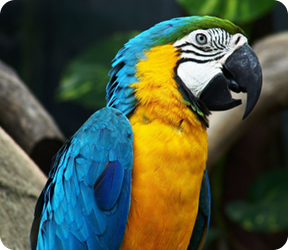
\includegraphics[width=0.9\textwidth]{figures/arara.png}\par}

\vspace{.7em}

\em Do you like araras? We do, specially our tool which shares the same name of this colorful bird.
\end{minipage}\hspace{1em}
\begin{minipage}{0.5\textwidth}
The tool name was chosen as an homage to a Brazilian bird of the same name, which is a macaw. The word \emph{arara} comes from the Tupian word \emph{a'rara}, which means \emph{big bird} (much to my chagrin, Sesame Street's iconic character Big Bird is not a macaw; according to some sources, he claims to be a golden condor). Araras are colorful, noisy, naughty and very funny. Everybody loves araras. The name seemed catchy for a tool and, in the blink of an eye, \arara\ was quickly spread to the whole \TeX\ world.
\end{minipage}
\end{messagebox}

Now that we informally introduced rules and directives, let us take a look on how \arara\ actually works given those two elements. The whole idea is pretty straightforward, and I promise to revisit these concepts later on in this manual for an comprehensive explanation (more precisely, on Chapter~\ref{chap:importantconcepts}).

First and foremost, we need to add at least one instruction in the source code to tell \arara\ what to do. This instruction is named \emph{directive} and it will be parsed during the preparation phase. Observe that \arara\ will tell you if no directive was found in a file, as seen in our first interaction with the tool.

An \arara\ directive is usually defined in a line of its own, started with a comment (denoted by a percent sign in \TeX\ and friends), followed by the word \abox{arara:} and task name:

\begin{codebox}{A typical directive}{teal}{\icnote}{white}
% arara: pdflatex
\documentclass{article}
...
\end{codebox}

Our example has one directive, referencing \abox{pdflatex}. It is important to observe that the \abox{pdflatex} identifier \emph{does not represent the command to be executed}, but \emph{the name of the rule associated with that directive}.

\begin{messagebox}{New feature in version 4.0}{araracolour}{\icinfo}{white}
\textbf{Multiline directives} -- Later on in Section~\ref{sec:directives} (page~\pageref{sec:directives}), we will discover that a directive can also span several lines in order to provide a better code organization. For now, let us assume a typical directive occupies only one line.
\end{messagebox}

Once \arara\ finds a directive, it will look for the associated \emph{rule}. In our example, it will look for a rule named \abox{pdflatex} which will evidently run the \abox{pdflatex} command line application. Rules are YAML files named according to their identifiers followed by the \abox{yaml} extension and follow a strict structure. This concept is covered in Section~\ref{sec:rule} (page~\pageref{sec:rule}).

\begin{messagebox}{New feature in version 4.0}{araracolour}{\icattention}{white}
\textbf{\gls{REPL} workflow} -- \arara\ now employs a \gls{REPL} workflow for rules and directives. In previous versions, directives were extracted, their corresponding rules were analized, commands were built and added to a queue before any proper execution or evaluation. I decided to change this workflow, so now \arara\ evaluates each rule on demand, that is, there is no \emph{a priori} checking. A rule will \emph{always} reflect the current state, including potential side effects from previous executed rules.
\end{messagebox}

Now, we have a queue of pairs $(\textit{directive}, \textit{rule})$ to process. For each pair, \arara\ will map the directive to its corresponding rule, evaluate it and run the proper command. The execution chain requires that command $i$ was successfully executed to then proceed to command $i+1$, and so forth. This is also by design: \arara\ will halt the execution if any of the commands in the queue had raised an error. How does one know if a command was successfully executed? \arara\ checks the corresponding \emph{exit status} available after a command execution. In general, a successful execution yields 0 as its exit status.

\begin{messagebox}{New feature in version 4.0}{araracolour}{\icinfo}{white}
\textbf{Custom exit status checking} -- In previous versions, there was no way of customizing the exit status checking of a command. A command was successful if, and only if, its resulting exit status was 0 and no other value. From now on, we can define any value, or even forget about it and make it always return a valid status regardless of execution (for instance, in a rule that always is successful -- see, for instance, the \abox{clean}  rule).
\end{messagebox}

That is pretty much how \arara\ works: directives in the source code are mapped to rules. These pairs are added to a queue. The queue is then executed and the status is reported. More details about the expansion process are presented in Chapter~\ref{chap:importantconcepts} (page~\pageref{chap:importantconcepts}). In short, we teach \arara\ to do a task by providing a rule, and tell it to execute it through directives in the source code.

\section{Operating system remarks}
\label{sec:operatingsystemremarks}

The application is written using the Java language, so \arara\ runs on top of a Java virtual machine, available on all the major operating systems~--~in some cases, you might need to install the proper virtual machine. We tried very hard to keep both code and libraries compatible with older virtual machines or from other vendors. Currently, \arara\ is known to run on Oracle's Java 5 to 10, and OpenJDK 5 to 10. We also have reports of users successfully using the tool with virtual machines provided by Azul Systems, so your mileage might vary greatly.

\begin{messagebox}{Outdated Java virtual machines}{attentioncolour}{\icerror}{black}
Dear reader, beware of outdated software, mainly Java virtual machines! Although \arara\ offers support for older virtual machines, try your best to keep your software updated as frequently as possible. The legacy support exists only for historical reasons, and also due to the sheer fact that we know some people that still runs \arara\ on very old hardware. If you are not in this particular scenario, get the latest virtual machine.
\end{messagebox}

In Chapter~\ref{chap:buildingfromsource} (page~\pageref{chap:buildingfromsource}), we provide instructions on how to build \arara\ from sources using Apache Maven. Even if you use multiple operating systems, \arara\ should behave the same, including the rules. There are helper functions available in order to provide support for system-specific rule based on the underlying operating system.

\section{Support}
\label{sec:support}

If you run into any issue with \arara, please let us know. We all have very active profiles in the \href{https://tex.stackexchange.com/}{\TeX\ community at StackExchange}, so just use the \abox{arara} tag in your question and we will help you the best we can (also, take a look at their \href{https://tex.meta.stackexchange.com/q/1436}{starter guide}).  We also have a \href{https://gitter.im/cereda/arara}{Gitter chat room}, in which we occasionally hang out. Also, you if you think the report is worthy of an issue, open one in our \href{https://github.com/cereda/arara/issues}{GitHub repository}. At last, but not least, feel free to poke us by good old electronic mail (please try the other approaches first).

We really hope you like our humble contribution to the \TeX\ community. Let \arara\ enhance your \TeX\ experience, it will help you when you will need it the most. Enjoy the manual.


\part{The application}
\label{part:application}

% !TeX root = ../arara-manual.tex
\chapter{Important concepts}
\label{chap:importantconcepts}

Time for our first proper contact with \arara! I must stress that is very important to understand a few concepts in which \arara\ relies before we proceed to the usage itself. Do not worry, these concepts are easy to follow, yet they are vital to the comprehension of the application and the logic behind it.

\section{Rules}
\label{sec:rule}

A \emph{rule} is a formal description of how \arara\ handles a certain task. For instance, if we want to use \rbox{pdflatex} with our tool, we should have a rule for that. Directives are mapped to rules, so a call to a non-existent rule \rbox{foo}, for instance, will indeed raise an error:

\begin{codebox}{Terminal}{teal}{\icnote}{white}
  __ _ _ __ __ _ _ __ __ _ 
 / _` | '__/ _` | '__/ _` |
| (_| | | | (_| | | | (_| |
 \__,_|_|  \__,_|_|  \__,_|

Processing 'doc1.tex' (size: 83 bytes, last modified: 05/03/2018
12:10:33), please wait.

I could not find a rule named 'foo' in the provided rule paths.
Perhaps a misspelled word? I was looking for a file named
'foo.yaml' in the following paths in order of priority:
(/opt/paulo/arara/rules)

Total: 0.09 seconds
\end{codebox}

Once a rule is defined, \arara\ automatically provides an access layer to that rule through directives in the source code, a concept to be formally introduced later on, in Section~\ref{sec:directives}. Observe that a directive reflects a particular instance of a rule of the same name (i.e, a \rbox{foo} directive in a certain source code is an instance of the \rbox{foo} rule).

In short, a rule is a plain text file written in the \gls{YAML} format, described in Chapter~\ref{chap:yaml}, on page~\pageref{chap:yaml}. I opted for this format because back then it was cleaner and more intuitive to use than other markup languages such as XML, besides of course being a data serialization standard for programming languages.

\begin{messagebox}{Animal jokes}{araracolour}{\icok}{white}
As a bonus, the acronym \emph{YAML} rhymes with the word \emph{camel}, so \arara\ is heavily environmentally friendly. Speaking of camels, there is the programming reference as well, since this amusing animal is usually associated with Perl and friends.
\end{messagebox}

The default rules, i.e, the rules shipped with \arara, are placed inside a special subdirectory named \abox[araracolour]{rules/} inside another special directory named \abox[araracolour]{ARARA\_HOME} (the place where our tool is installed). We will learn later on, in Section~\ref{sec:basicstructure}, on page~\pageref{sec:basicstructure}, that we can add an arbitrary number of paths for storing our own rules, in order of priority, so do not worry too much about the location of the default rules, although it is important to understand and acknowledge their existence.

The following list describes the basic structure of an \arara\ rule by presenting the proper elements (or keys, if we consider the proper \gls{YAML} nomenclature). Observe that elements marked as \rbox[araracolour]{M} are mandatory (i.e, the rule \emph{has} to have them in order to work). Similarly, elements marked as \rbox[araracolour]{O} are optional, so you can safely ignore them when writing a rule for our tool. A key preceded by \rbox{context$\rightarrow$} indicates a context and should be properly defined inside it.

\begin{description}
\item[\describe{M}{!config}] This keyword is mandatory and must be the first line of any \arara\ rule. It denotes the object mapping metadata to be internally used by the tool. Actually, the tool is not too demanding on using it (in fact, you could suppress it entirely and \arara\ will not complain), but it is considered good practice to start all rules with a \abox{!config} keyword regardless.

\item[\describe{M}{identifier}] This key acts as a unique identifier for the rule (as expected). It is highly recommended to use lowercase letters without spaces, accents or punctuation symbols, as good practice (again). As a convention, if you have an identifier named \rbox{pdflatex}, the rule filename must be \rbox{pdflatex.yaml} (like our own instance). Please note that, although \rbox{yml} is known to be a valid \gls{YAML} extension as well, \arara\ only considers files ending with the \rbox{yaml} extension. This is a deliberate decision.

\begin{codebox}{Example}{teal}{\icnote}{white}
identifier: pdflatex
\end{codebox}

\item[\describe{M}{name}] This key holds the name of the \emph{task} (a rule instantiated through a directive) as a plain string. When running \arara, this value will be displayed in the output enclosed in parentheses.

\begin{codebox}{Example}{teal}{\icnote}{white}
name: PDFLaTeX
\end{codebox}

\item[\describe{O}{authors}] We do love blaming people, so \arara\ features a special key to name the rule authors (if any) so you can write stern electronic communications to them! This key holds a list of strings. If the rule has just one author, add it as the first (and only) element of the list.

\begin{codebox}{Example}{teal}{\icnote}{white}
authors:
- Marco Daniel
- Paulo Cereda
\end{codebox}

\item[\describe{M}{commands}] This key is introduced in version 4.0 of \arara\ and denotes a potential list of commands. From the user perspective, each command is called a \emph{subtask} within a task (rule and directive) context. A task may represent only a single command (a single subtask), as well as a sequence of commands (subtasks). For instance, the \rbox{frontespizio} rule requires at least two commands. So, as a means of normalizing the representation, a task composed of a single command (single subtask) is defined as the only element of the list, as opposed to previous versions of \arara, which had a specific key to hold just one command.

\begin{messagebox}{Incompatibility with older versions}{attentioncolour}{\icerror}{black}
Dear reader, note that rules from version 4.0 are incompatible with older versions of \arara. If you are migrating from old versions to version 4.0, we need to replace \abox{command} by \abox{commands} and specify a contextual element, as seen in the following descriptions. Please refer to Section~\ref{sec:migrationguide}, on page~\pageref{sec:migrationguide}, for a comprehensible migration guide.
\end{messagebox}

In order to properly set a subtask, the keys used in this specification are defined inside the \rbox{commands$\rightarrow$} context and presented as follows.

\begin{description}
\item[\describecontext{O}{commands}{name}] This key holds the name of the subtask as a plain string. When running \arara, this value will be displayed in the output. Subtask names are displayed after the main task name. By the way, did you notice that this key is entirely optional? That means that a subtask can simply be unnamed, if you decide so. However, such practice is not recommended, as it's always good to have a visual description of what \arara\ is running at the moment, so name your subtasks properly.

\item[\describecontext{M}{commands}{command}] This key holds the action to be performed, typically a system command. In previous versions, \arara\ would rely solely on a string. For this version on, as a means to enhance the user experience (and also fix serious blockers when handling spaces in file names, as seen in \href{https://github.com/cereda/arara/issues}{previous issues} reported in the repository), the tool offers four types of returned values:

\begin{itemize}[label={--}]
\item A plain string: this is the default (and only) behaviour in older versions of \arara. The plain string is processed as it is by the underlying execution engine. However, automatic argument parsing is problematic, so this approach, although supported, is not recommended any more.

\begin{codebox}{Example}{teal}{\icnote}{white}
command: 'ls'
\end{codebox}

It is important to observe that you can use either a plain string directly or use an orb tag with an explicit \rbox{return} command (as seen in Section~\ref{sec:mvelbasicusage}, on page~\pageref{sec:mvelbasicusage}). Personally, I favour the explicit indication for a quick understanding.

\item A \rbox{Command} object: \arara\ 4.0 features a new approach for handling system commands based on a high level structure with explicit argument parsing named \rbox{Command} (for our curious users, it is a plain Java object). In order to use this approach, we need to rely on orb tags and use a helper method named \mtbox{getCommand} to obtain the desired result. We will detail this method later on, in Section~\ref{sec:commandsandtriggers}, on page~\pageref{sec:commandsandtriggers}. We highly recommend the adoption of this approach for rule writing instead of using plain strings.

\begin{codebox}{Example}{teal}{\icnote}{white}
command: "@{ return getCommand('ls') }"
\end{codebox}

\item A boolean value: it is also possible to exploit the expressive power of the underlying scripting language available in the rule context (see Chapter~\ref{chap:mvel}, on page~\pageref{chap:mvel}, for more details) for writing complex code. In this particular case, since the computation is being done by \arara\ itself and not the underlying operating system, there will not be a command to be executed, so simply return a boolean value -- either an explicit \rbox{true} or \rbox{false} value or a logical expression -- to indicate whether the computation was successful.

\begin{codebox}{Example}{teal}{\icnote}{white}
command: "@{ return 1 == 1 }"
\end{codebox}

\item A \rbox{Trigger} object: this is surely the least common type of returned value and it is mentioned here just for documentation purposes. In simple terms, a \rbox{Trigger} object constitutes a special command that changes the internal workings of \arara\ at runtime. We have not worked much on this concept, so there is only one trigger available, seen in action in the official \rbox{halt} rule. In order to use this approach, we need to rely on orb tags and use a helper method named \mtbox{getTrigger} to obtain the desired result.
\end{itemize}

It is also worth mentioning that \arara\ also supports lists of commands represented as plain strings, \rbox{Command} or \rbox{Trigger} objects, boolean values or a mix of them. This is useful if your rule has to decide whether more actions are required in order to accomplish a task. In this case, our tool will take care of the list and execute each element in the specified order.

\begin{codebox}{Example}{teal}{\icnote}{white}
command: "@{ return [ 'ls', 'ls', 'ls' ] }"
\end{codebox}

As an example, please refer to the official \rbox{clean} rule for a real scenario where a list of commands is successfully employed: for each provided extension, the rule creates a new cleaning command and adds it to a list of removals to be processed later.

\begin{messagebox}{Plain string is deprecated}{attentioncolour}{\icattention}{black}
It took me a lot of effort to find out that handling plain strings and employing guesswork to parse arguments are the root of several issues reported by users. Therefore, this approach is being marked as \emph{deprecated} and will be removed in future versions.
\end{messagebox}

There are at least two variables available in the \abox{command} context and are described as follows (note that \gls{MVEL} variables and orb tags are discussed in Chapter~\ref{chap:mvel}). A variable will be denoted by \varbox{variable} in this list. For each rule argument (defined later on), there will be a corresponding variable in the \abox{command} context, directly accessed through its unique identifier.

\begin{description}
\item[\varbox{file}] This variable holds the file name, without any path reference, as a plain string. It is usually composed from the base name and the extension. This variable is available since the first release of \arara.

\item[\varbox{reference}] This variable is introduced in version 4.0 of \arara\ and holds the canonical, absolute path representation of the \varbox{file} variable as a \rbox{File} object. This is useful if it's necessary to know the hierarchical structure of a project. Since the reference is a Java object, we can use all methods available in the \rbox{File} class.
\end{description}

\begin{messagebox}{Quote handling}{araracolour}{\icinfo}{white}
\setlength{\parskip}{1em}
The \gls{YAML} format disallows key values starting with \rbox{@} without proper quoting. This is the reason we had to use double quotes for the value and internally using single quotes for the command string. Also, we could use the other way around, or even using only one type and then escaping them when needed. This is excessively verbose but needed due to the format requirement. Thankfully, \arara\ offers two solutions for removing the quoting verbosity when writing commands.

The first solution is used in previous versions and it still works like a charm in modern days. We need to precede our command with a special keyword \rbox{<arara>} which will be removed afterwards. This solution works on virtually every key in the rule context, so it is a bonus. The new code will look like this:

\begin{codebox}{Example}{teal}{\icnote}{white}
command: <arara> @{ return getCommand('ls') }
\end{codebox}

The second approach is more of a \gls{YAML} feature rather than a tool exclusive, although we have to do a couple of checks under the hood in order to ensure the correct execution. The idea here is to use the scalar content in folded style, as seen in Section~\ref{sec:yamlscalars}, on page~\pageref{sec:yamlscalars}. The new code will look like this:

\begin{codebox}{Example}{teal}{\icnote}{white}
command: >
  @{
    return getCommand('ls')
  }
\end{codebox}

Mind the indentation, as \gls{YAML} requires it to properly identify blocks. I personally recommend this approach for longer code, as it provides a better visual representation. You will see the second solution all around the default rules, but feel free to use the one you feel more comfortable with.
\end{messagebox}

\item[\describecontext{O}{commands}{exit}] This key holds a special purpose in \arara\ 4.0, as it represents a custom exit status evaluation for the corresponding command. In general, a successful execution has zero as an exit status, but sometimes we end up with tools or situations where we need to override this check for whatever reason. For this purpose, simply write a \gls{MVEL} expression \emph{without orb tags} as plain string and use the special variable \varbox{value} if you need the actual exit status returned by the command, available at runtime. For example, if the command returns a non-zero value indicating a successful execution, we can write this key as:

\begin{codebox}{Example}{teal}{\icnote}{white}
exit: value > 0
\end{codebox}

If the execution should be marked as successful by \arara\ regardless of the actual exit status, you can simply write \rbox{true} as the key value and this rule will never fail, for obvious reasons.
\end{description}

For instance, consider a full example of the \abox{commands} key, defined with only one command, presented as follows. The hyphen denotes a list element, so mind the indentation for correctly specifying the component keys. Also, note that, in this case, the \abox{exit} key was completely optional, as it does the default checking, and it was included for didactic purposes.

\begin{codebox}{Example}{teal}{\icnote}{white}
commands:
- name: The PDFLaTeX engine
  command: >
    @{
      return getCommand('pdflatex', file)
    }
  exit: value == 0
\end{codebox}

\item[\describe{M}{arguments}] This key holds a list of arguments for the current rule, if any. The arguments specified in this list will be available to the user later on for potential completion through directives. Once instantiated, they will become proper variables in the \abox{command} contexts. This key is mandatory, so even if your rule does not have arguments, you need to specify a list regardless. In this case, use the empty list notation:

\begin{codebox}{Example}{teal}{\icnote}{white}
arguments: []
\end{codebox}

In order to properly set an argument, the keys used in this specification are defined inside the \rbox{arguments$\rightarrow$} context and presented as follows.

\begin{description}
\item[\describecontext{M}{arguments}{identifier}] This key acts as a unique identifier for the argument. It is highly recommended to use lowercase letters without spaces, accents or punctuation symbols, as a good practice. This key will be used later on to set the corresponding value in the directive context.

\begin{codebox}{Example}{teal}{\icnote}{white}
identifier: shell
\end{codebox}

It is important to mention that not all names are valid as argument identifiers. \arara\ has restrictions on three names, described as follows, which cannot be used.

\begin{messagebox}{Reserved names for rule arguments}{attentioncolour}{\icattention}{black}
Our tool has three names reserved for internal use: \abox{file}, \abox{files}, and \abox{reference}. Do not use them as argument identifiers!
\end{messagebox}

\item[\describecontext{O}{arguments}{flag}] This key holds a plain string and is evaluated when the corresponding argument is defined in the directive context.  After being evaluated, the result will be stored in a variable of the same name to be later accessed in the \abox{command} context. In the scenario where the argument is not defined in the directive, the variable will hold an empty string.

\begin{codebox}{Example}{teal}{\icnote}{white}
flag: >
  @{
      isTrue(parameters.shell, '--shell-escape',
             '--no-shell-escape')
  }
\end{codebox}

There are three variables available in the \abox{flag} context, described as follows. Note that are also several helper methods available in the rule context (for instance, \mtbox{isTrue} presented in the previous example) which provide interesting features for rule writing. They are detailed later on, in Chapter~\ref{chap:methods}, on page~\pageref{chap:methods}.

\begin{description}
\item[\varbox{parameters}] This variable holds a map of directive parameters available at runtime. For each argument identifier listed in the \abox{arguments} list in the rule context, there will be an entry in this variable. This is useful to get the actual values provided during execution and take proper actions. If a parameter is not set in the directive context, the reference will still exist in the map, but it will be mapped to an empty string.

\item[\varbox{file}] This variable holds the file name, without any path reference, as a plain string. It is usually composed from the base name and the extension. This variable is available since the first release of \arara.

\item[\varbox{reference}] This variable is introduced in version 4.0 of \arara\ and holds the canonical, absolute path representation of the \varbox{file} variable as a \rbox{File} object. This is useful if it's necessary to know the hierarchical structure of a project. Since the reference is a Java object, we can use all methods available in the \rbox{File} class.
\end{description}

In the previous example, observe that the \gls{MVEL} expression defined in the \abox{flag} key checks if the user provided an affirmative value regarding shell escape, through comparing \varbox{parameters.shell} with a set of predefined affirmative values. In any case, the corresponding command flag is defined as result of such evaluation.

\item[\describecontext{O}{arguments}{default}] As default behaviour, if a parameter is not set in the directive context, the reference will be mapped to an empty string. This key exists for the exact purpose of overriding such behaviour.

\begin{codebox}{Example}{teal}{\icnote}{white}
default: ''
\end{codebox}

There are three variables available in the \abox{default} context, described as follows. Note that are also several helper methods available in the rule context (for instance, \mtbox{isTrue} presented in the previous example) which provide interesting features for rule writing. They are detailed later on, in Chapter~\ref{chap:methods}, on page~\pageref{chap:methods}.

\begin{description}
\item[\varbox{parameters}] This variable holds a map of directive parameters available at runtime. For each argument identifier listed in the \abox{arguments} list in the rule context, there will be an entry in this variable. This is useful to get the actual values provided during execution and take proper actions. If a parameter is not set in the directive context, the reference will still exist in the map, but it will be mapped to an empty string.

\item[\varbox{file}] This variable holds the file name, without any path reference, as a plain string. It is usually composed from the base name and the extension. This variable is available since the first release of \arara.

\item[\varbox{reference}] This variable is introduced in version 4.0 of \arara\ and holds the canonical, absolute path representation of the \varbox{file} variable as a \rbox{File} object. This is useful if it's necessary to know the hierarchical structure of a project. Since the reference is a Java object, we can use all methods available in the \rbox{File} class.
\end{description}

\item[\describecontext{O}{arguments}{required}] There might be certain scenarios in which a rule could make use of required arguments (for instance, a copy operation in which source and target must be provided). The \abox{required} key acts as a boolean switch to indicate whether the corresponding argument should be mandatory. In this case, set the key value to \rbox{true} and the argument becomes required. Later on at runtime, \arara\ will throw an error if a required parameter is missing in the directive.

\begin{codebox}{Example}{teal}{\icnote}{white}
required: false
\end{codebox}

Note that setting the \abox{required} key value to \rbox{false} corresponds to omitting the key completely in the rule context, which resorts to the default behaviour (i.e, all arguments are optional).
\end{description}

\begin{messagebox}{Note on argument keys}{attentioncolour}{\icattention}{black}
As seen previously, both \abox{flag} and \abox{default} are marked as optional, but at least one of them must occur in the argument specification, otherwise \arara\ will throw an error, as it makes no sense to have no argument handling at all. Please make sure to specify at least one of them for a consistent behaviour!
\end{messagebox}

For instance, consider a full example of the \abox{arguments} key, defined with only one argument, presented as follows. The hyphen denotes a list element, so mind the indentation for correctly specifying the component keys. Also, note that, in this case, keys \abox{required} and \abox{default} were completely optional, and they were included for didactic purposes.

\begin{codebox}{Example}{teal}{\icnote}{white}
arguments:
- identifier: shell
  flag: >
    @{
        isTrue(parameters.shell,
               '--shell-escape',
               '--no-shell-escape')
    }
  required: false
  default: ''
\end{codebox}
\end{description}

This is the rule structure in the \gls{YAML} format used by \arara. Keep in mind that all subtasks in a rule are checked against their corresponding exit status. If an abnormal execution is detected, the tool will instantly halt and the rule will fail. Even \arara\ itself will return an exit code different than zero when this situation happens (detailed in Chapter~\ref{chap:commandline}, on page~\pageref{chap:commandline}).

\section{Directives}
\label{sec:directives}

A \emph{directive} is a special comment inserted in the source file in which you indicate how \arara\ should behave. You can insert as many directives as you want and in any position of the file. The tool will read the whole file and extract the directives.

\begin{messagebox}{New features in version 4.0}{araracolour}{\icinfo}{white}
\setlength{\parskip}{1em}
\textbf{Partial directive extraction} -- From version 4.0 of \arara\ on, it is now possible to extract directives only available in the file preamble, i.e, all lines from the beginning that are comments until reaching the first line that is not a comment (excluding blank lines). To this end, a new command line flag is introduced in Section~\ref{sec:basicstructure}, on page~\pageref{sec:basicstructure}.

\textbf{Predefined preambles} -- Common preambles can be predefined and used with files that require the same automation steps, then \arara\ can be invoked based on such specifications. This feature is covered in Section~\ref{sec:basicstructure}, on page~\pageref{sec:basicstructure}.
\end{messagebox}


There are two types of directives in \arara\ which determine the way the corresponding rules will be instantiated. They are listed as follows. Note that directives are always preceded by the \rbox{arara:} pattern.

\begin{description}
\item[empty directive] This type of directive has already been mentioned in Chapter~\ref{chap:introduction}, on page~\pageref{chap:introduction}, it has only the rule name (which refers to the \abox{identifier} key from the rule of the same name). All rule arguments are mapped to empty strings, except the ones with \abox{default} values.

\begin{codebox}{Empty directive}{teal}{\icnote}{white}
% arara: pdflatex
\end{codebox}

\item[parametrized directive] This type of directive also has the rule name (which refers to the \abox{identifier} key from the rule of the same name), and also contains a map of parameters in order to provide additional information to the corresponding rule. This map is defined in the \gls{YAML} format, based on the inline style.

\begin{codebox}{Parametrized directive}{teal}{\icnote}{white}
% arara: pdflatex: { shell: yes }
\end{codebox}

Observe that \arara\ relies on named parameters, so they are mapped by their corresponding argument identifiers and not by their positions. The syntax for a parameter is described as follows. Please refer to the map definition in Section~\ref{sec:yamlcollections}, on page~\pageref{sec:yamlcollections}.

\begin{codebox}{Parameter syntax}{teal}{\icnote}{white}
key : value
\end{codebox}

Note that virtually any type of data can be used as parameter value, so lists, integers, booleans, sets and other maps are available as well. However, there must be the correct handling of such types in the rule context.
\end{description}

When handling parametrized directives, \arara\ always checks if directive parameters and rule arguments match. If we try to inject a non-existent parameter in a parametrized directive, the tool will raise an error about it:

\begin{codebox}{Terminal}{teal}{\icnote}{white}
  __ _ _ __ __ _ _ __ __ _ 
 / _` | '__/ _` | '__/ _` |
| (_| | | | (_| | | | (_| |
 \__,_|_|  \__,_|_|  \__,_|

Processing 'hello.tex' (size: 103 bytes, last modified:
05/03/2018 15:40:16), please wait.

I have spotted an error in rule 'pdflatex' located at
'/opt/paulo/arara/rules'. I found these unknown keys
in the directive: (foo). This should be an easy fix,
just remove them from your map.

Total: 0.21 seconds
\end{codebox}

As the message suggests, we need to remove the unknown parameter key from our directive or rewrite the rule in order to include it as an argument. The first option is, of course, easier.

\begin{messagebox}{New feature in version 4.0}{araracolour}{\icinfo}{white}
\textbf{Helpful messages} -- It is a staple of \arara\ to have friendly and helpful messages. From version 4.0 on, we decided to make messages even friendlier and include suggestions for correcting errors or improving usage. So, whenever possible, make sure to read all messages our tool provides, they will help you!
\end{messagebox}

Sometimes, directives can span several columns of a line, particularly the ones with several parameters. From \arara\ 4.0 on, we can split a directive into multiple lines by using the \rbox{arara: {-}{-}>} mark (also known as \emph{arrow notation} during development) to each line which should compose the directive. We call it a \emph{multiline directive}. Let us see an example:

\begin{codebox}{Multiline directive}{teal}{\icnote}{white}
% arara: pdflatex: {
% arara: --> shell: yes,
% arara: --> synctex: yes
% arara: --> }
\end{codebox}

It is important to observe that there is no need of them to be in contiguous lines, i.e, provided that the syntax for parametrized directives hold for the line composition, lines can be distributed all over the code. In fact, the log file (when enabled) will contain a list of all line numbers that compose a directive. This feature is discussed later on, in Section~\ref{sec:directiveextraction}, on page~\pageref{sec:directiveextraction}.

\begin{messagebox}{Keep lines together}{araracolour}{\icinfo}{white}
Although it is possible to spread lines of a multiline directive all over the code, it is considered good practice to keep them together for easier reading and editing. In any case, you can always see which lines compose a directive by inspecting the log file.
\end{messagebox}

\arara\ 4.0 provides logical expressions, written in the \gls{MVEL} language, and special operators processed at runtime in order to determine whether and how a directive should be processed. This feature is named \emph{directive conditional}, or simply \emph{conditional} as an abbreviation. The following list describes all conditional operators available in the directive context.

\begin{description}
\item[\describeconditional{a priori}{if}] The associated \gls{MVEL} expression is evaluated beforehand, and the directive is interpreted if, and only if, the result of such evaluation is true. This directive, when the conditional holds true, is executed at most once.

\begin{codebox}{Conditional}{teal}{\icnote}{white}
% arara: pdflatex if missing('pdf') || changed('tex')
\end{codebox}

\item[\describeconditional{a posteriori}{until}] The directive is interpreted the first time, then the associated \gls{MVEL} expression evaluation is done. While the result holds false, the directive is interpreted again and again. There are no guarantees of proper halting.

\begin{codebox}{Conditional}{teal}{\icnote}{white}
% arara: pdflatex until !found('log', 'undefined references')
\end{codebox}

\item[\describeconditional{a priori}{unless}] Technically an inverted \cdbox{if} conditional, the associated \gls{MVEL} expression is evaluated beforehand, and the directive is interpreted if, and only if, the result is false. This directive, when the conditional holds false, is executed at most once.

\begin{codebox}{Conditional}{teal}{\icnote}{white}
% arara: pdflatex unless unchanged('tex') && exists('pdf')
\end{codebox}

\item[\describeconditional{a priori}{while}] The associated \gls{MVEL} expression is evaluated beforehand, the directive is interpreted if, and only if, the result is true, and the process is repeated while the result still holds true. There are no guarantees of proper halting.

\begin{codebox}{Conditional}{teal}{\icnote}{white}
% arara: pdflatex while missing('pdf') ||
% arara: --> found('log', 'undefined references')
\end{codebox}
\end{description}

Several methods are available in the directive context in order to ease the writing of conditionals, such as \mtbox{missing}, \mtbox{changed}, \mtbox{found}, \mtbox{unchanged}, and \mtbox{exists} featured in the previous examples. They will be properly detailed later on, in Section~\ref{sec:files}, on page~\pageref{sec:files}.

\begin{messagebox}{No infinite loops}{araracolour}{\icinfo}{white}
Although there are no conceptual guarantees for proper halting of unbounded loops, we have provided a technical solution for potentially infinite iterations: \arara\ has a predefined maximum number of loops. The default value is set to 10, but it can be overridden either in the configuration file or with a command line flag. We discuss this feature later on, in Sections~\ref{sec:options} and~\ref{sec:basicstructure}, on pages~\pageref{sec:options} and~\pageref{sec:basicstructure}, respectively.
\end{messagebox}

All directives, regardless of their type, are internally mapped with both \abox{file} and \abox{reference} parameters, discussed earlier on, in Section~\ref{sec:coreconcepts}, on page~\pageref{sec:coreconcepts}, as special variables in the rule context. When inspecting the log file, you will find all map keys and values for each extracted directive (actually, there is an entire log section devoted to detailing directives found in the code). This feature is covered in Section~\ref{sec:directivenormalization}, on page~\pageref{sec:directivenormalization}. See, for instance, the report of the directive extraction and normalization process performed by \arara\ when inspecting \rbox{doc2.tex}, available in the log file. Note that timestamps were deliberately removed in order to declutter the output, and line breaks were included in order to easily spot the log entries.

\begin{ncodebox}{Source file}{teal}{\icnote}{white}{doc2.tex}
% arara: pdflatex
% arara: pdflatex: { shell: yes }
\documentclass{article}

\begin{document}
Hello world.
\end{document}
\end{ncodebox}

\begin{codebox}{An excerpt of the log file (directive section)}{teal}{\icnote}{white}
Directive: { identifier: pdflatex, parameters:
{reference=/home/paulo/doc2.tex, file=doc2.tex},
conditional: { NONE }, lines: [1] }

Directive: { identifier: pdflatex, parameters:
{shell=yes, file=doc2.tex, reference=/home/paulo/doc2.tex},
conditional: { NONE }, lines: [2] }
\end{codebox}

The directive context also features another special parameter named \abox{files} which expects a non-empty list of file names as plain string values. For each element of this list, \arara\ will replicate the current directive and point the element being iterated as current \abox{file} and \abox{reference} values (being the latter resolved to a proper absolute, canonical path of the former). See, for instance, the report of the directive extraction and normalization process performed by \arara\ when inspecting \rbox{doc3.tex}, available in the log file.

\begin{ncodebox}{Source file}{teal}{\icnote}{white}{doc3.tex}
% arara: pdflatex: { files: [ doc1.tex, doc2.tex ] }
Hello world.
\bye
\end{ncodebox}

\begin{codebox}{An excerpt of the log file (directive section)}{teal}{\icnote}{white}
Directive: { identifier: pdflatex, parameters:
{reference=/home/paulo/doc1.tex, file=doc1.tex},
conditional: { NONE }, lines: [1] }

Directive: { identifier: pdflatex, parameters:
{reference=/home/paulo/doc2.tex, file=doc2.tex},
conditional: { NONE }, lines: [1] }
\end{codebox}

In this case \rbox{doc3.tex} is a plain \TeX\ file, but \rbox{pdflatex} is actually being called on two \LaTeX\ documents, first \rbox{doc1.tex} and then \rbox{doc2.tex}.

Even when a directive is interpreted with a file other than the one being processed by \arara\ (through the magic of the \abox{files} parameter), it is possible to use helper methods in the rule context to get access to the original file and reference. Such methods are detailed later on, in Section~\ref{sec:files}, on page~\pageref{sec:files}.

\section{Migration guide}
\label{sec:migrationguide}

\begin{messagebox}{A note to users}{araracolour}{\icattention}{white}
If this is your first time using \arara\ or you do not have custom rules in the old format, you can safely ignore this section. All rules shipped with our tool are already written in the new format.
\end{messagebox}

As previously discussed in Section~\ref{sec:rule}, on page~\pageref{sec:rule}, version 4.0 of \arara\ introduces a new rule format. As a result, user-defined rules in the old format are incompatible with the new version of our tool and thus have to be updated. In short, we need to replace \abox{command} by \abox{commands} and specify a contextual element. As an example, consider the following hypothetical rule \rbox{ls} written in the old format:

\begin{codebox}{A rule in the old format}{teal}{\icnote}{white}
!config
identifier: ls
name: LS
command: ls @{details}
arguments:
- identifier: details
  flag: '@{ isTrue(parameters.details, "-l", "") }'
\end{codebox}

This rule does nothing too important, it simply runs the system command \rbox{ls} which lists the contents of the current directory. However, when we try to run \arara\ on a file which contains a directive referencing this rule, we get the following error in the terminal:

\begin{codebox}{Terminal}{teal}{\icnote}{white}
  __ _ _ __ __ _ _ __ __ _ 
 / _` | '__/ _` | '__/ _` |
| (_| | | | (_| | | | (_| |
 \__,_|_|  \__,_|_|  \__,_|

Processing 'doc4.tex' (size: 31 bytes, last modified: 05/27/2018
21:05:57), please wait.

I have spotted an error in rule 'ls' located at '/home/paulo'. I
could not parse the rule, something bad happened. Apparently, the
provided YAML file is invalid. I will do my best to help you in
any way I can. There are more details available on this
exception:

DETAILS ---------------------------------------------------------
Cannot create property=command for
JavaBean=com.github.cereda.arara.model.Rule@29774679
 in
'reader', line 1, column 1:
    !config
    ^
Unable to find
property 'command' on class: com.github.cereda.arara.model.Rule

in 'reader', line 4, column 10:
    command: ls @{details}
      
      ^


Total: 0.03 seconds
\end{codebox}

The above terminal output shows the usual error \arara\ raises when a rule in the old format is used, and thus the corresponding \gls{YAML} file is considered invalid. In order to fix the rule, we need to move the \abox{command} key inside a \rbox{commands$\rightarrow$} context as a list element, as seen as follows.

\begin{codebox}{A rule converted into the new format}{teal}{\icnote}{white}
!config
identifier: ls
name: LS
commands:
- command: ls @{details}
arguments:
- identifier: details
  flag: '@{ isTrue(parameters.details, "-l", "") }'
\end{codebox}

Note that this fix is sufficient to make the rule valid in the new format. Also, it is interesting to observe that the subtask will be unnamed during the execution, as there is no corresponding \abox{name} key  in the list element.

\begin{codebox}{Terminal}{teal}{\icnote}{white}
(LS) Unnamed task ....................................... SUCCESS
\end{codebox}

Now, let us consider an example containing a list of commands, also based on the old format. The \rbox{ls} rule was updated to include two runs of the system command of the same name in the current directory:

\begin{codebox}{A rule in the old format}{teal}{\icnote}{white}
!config
identifier: ls
name: LS
commands:
- ls @{details}
- ls @{details}
arguments:
- identifier: details
  flag: '@{ isTrue(parameters.details, "-l", "") }'
\end{codebox}

Observe that the old format directly represents commands as a list of plain strings. When trying to run \arara\ on a file which contains a directive referencing the updated \rbox{ls} rule, we get the following error in the terminal:

\begin{codebox}{Terminal}{teal}{\icnote}{white}
  __ _ _ __ __ _ _ __ __ _ 
 / _` | '__/ _` | '__/ _` |
| (_| | | | (_| | | | (_| |
 \__,_|_|  \__,_|_|  \__,_|

Processing 'doc4.tex' (size: 31 bytes, last modified: 05/27/2018
21:05:57), please wait.

I have spotted an error in rule 'ls' located at '/home/paulo'. I
could not parse the rule, something bad happened. Apparently, the
provided YAML file is invalid. I will do my best to help you in
any way I can. There are more details available on this
exception:

DETAILS ---------------------------------------------------------
Cannot create property=commands for
JavaBean=com.github.cereda.arara.model.Rule@91161c7
 in 'reader',
line 1, column 1:
    !config
    ^
No single argument
constructor found for class
com.github.cereda.arara.model.RuleCommand
 in 'reader', line 5,
column 1:
    - ls @{details}
    ^


Total: 0.02 seconds
\end{codebox}

The above terminal output shows a slightly different message, but the error is practically the same to the one \arara\ raised before when a rule in the old format was used. The difference relies on the missing rule property being set at the moment, but the idea remains the same. In order to fix the rule, we need to precede every list element in the \rbox{commands$\rightarrow$} context with the \abox{command} key, as seen as follows.

\begin{codebox}{A rule converted into the new format}{teal}{\icnote}{white}
!config
identifier: ls
name: LS
commands:
- command: ls @{details}
- command: ls @{details}
arguments:
- identifier: details
  flag: '@{ isTrue(parameters.details, "-l", "") }'
\end{codebox}

This fix is sufficient to make the rule valid in the new format. Also, as mentioned before, it is interesting to observe that the subtasks will be unnamed during the execution, as there are no corresponding \abox{name} keys in the list elements.

\begin{codebox}{Terminal}{teal}{\icnote}{white}
(LS) Unnamed task ....................................... SUCCESS
(LS) Unnamed task ....................................... SUCCESS
\end{codebox}

There is a helper tool available in the \href{https://github.com/cereda/arara/releases/tag/4.0}{release section} of our project repository that attempts to automatically convert rules in the old format to the new one. If you want to try it, download the \rbox{rc.jar} file from the repository and put it in the same directory where the old rules are located. You can also provide a full path instead. It is important to note that, although the tool might indicate a successful conversion, there are no guarantees that the resulting rule is fully compliant with the new format, due to potential changes in the internal workings of \arara, so your mileage may vary. In general, it should work. The rule converter is written in Java and requires a virtual machine to run. The tool has a straightforward workflow and takes just one parameter referring to the rule to be converted. The entire process should happen without intervention. When invoked without the file name, this is the expected output:

\begin{codebox}{Terminal}{teal}{\icnote}{white}
$ java -jar rc.jar
         _                                _
 ___ _ _| |___    ___ ___ ___ _ _ ___ ___| |_ ___ ___
|  _| | | | -_|  |  _| . |   | | | -_|  _|  _| -_|  _|
|_| |___|_|___|  |___|___|_|_|\_/|___|_| |_| |___|_|

version 1.0 (rules < 4.0)

OH NO! -----------------------------------------------------
This tool expects the YAML rule from previous versions of
arara. Please, provide a proper YAML file containing the old
rule as a parameter and try again. I will do my best to
convert the rule to the new version 4.0 format.
\end{codebox}

Let us invoke the tool with the first version of our hypothetical \rbox{ls} rule, still in the old format. The tool removes all comments from the original file, if any, and constructs a new file with a \rbox{\_v4} suffix attached to the name. The original file is preserved. Just keep in mind that the new rule must be renamed afterwards, as the base name and the corresponding \abox{identifier} key must match. The output is presented as follows.

\begin{codebox}{Terminal}{teal}{\icnote}{white}
$ java -jar rc.jar ls.yaml
         _                                _
 ___ _ _| |___    ___ ___ ___ _ _ ___ ___| |_ ___ ___
|  _| | | | -_|  |  _| . |   | | | -_|  _|  _| -_|  _|
|_| |___|_|___|  |___|___|_|_|\_/|___|_| |_| |___|_|

version 1.0 (rules < 4.0)

The provided YAML rule looks OK. I will try my best to
convert it to the new version 4.0 format adopted by arara.
The new rule name will be written in the same directory of
the original one and will have a '_v4' suffix to it. Keep in
mind that the base name must match the identifier!

YAY! -------------------------------------------------------
Good news, everybody! The provided YAML rule was updated
successfully to the new version 4.0 format of arara! Of
course, there are no guarantees this new rule will work out
of the box, so fingers crossed! Take a closer look at the
manual and update your rule to use the new enhancements of
arara. Have a great time!
\end{codebox}

The resulting rule is identical to the one manually converted in this section. Just note that, when creating the file, the resulting \gls{YAML} file might write the keys in alphabetical order. That means that, although both files semantically represent the same rule, the positions of the keys differ. However, that poses no issue at all, as long as the keys are correctly defined. Also, it is important to note that, due to a conversion policy of the underlying \gls{YAML} library, folded scalars in the old format are transcribed as literal scalars in the new format. We could force a folded style as default, but the resulting rule would be unnecessarily verbose, so we opted for the simpler, cleaner solution. As a direct consequence, we strongly recommend a subsequent verification and potential fix of existing literal scalars into folded ones, if any. Please refer to Section~\ref{sec:yamlscalars}, on page~\pageref{sec:yamlscalars}, for more details on scalars.

\begin{messagebox}{Replace plain strings in commands}{araracolour}{\icattention}{white}
As plain strings are known to be problematic when defining commands, they are marked as deprecated in version 4.0 of \arara\ and will likely be removed in future releases. Since you are migrating from an old format to a new one, please consider replacing plain strings in command by proper \rbox{Command} objects. The helper methods available in the rule context, including the indispensable \mtbox{getCommand} method, for obvious reasons, are detailed in Section~\ref{sec:commandsandtriggers}, on page~\pageref{sec:commandsandtriggers}. It is highly advisable to update your rules on this regard, if applicable.
\end{messagebox}

This section pretty much covered the basics for correctly migrating rules in the old format to the new one. Of course, it is highly advisable to make use of the new features available in \arara\ 4.0 for achieving better results. If you need any help, please do not hesitating in contacting us. See Section~\ref{sec:support}, on page~\pageref{sec:support}, for more details on how to get help.

% !TeX root = ../arara-manual.tex
\chapter{Command line}
\label{chap:commandline}

\arara\ is a command line tool. It can be used in a plethora of command interpreter implementations, from bash to a Windows prompt, provided that the Java runtime environment is accessible within the current session. This chapter covers the user interface design, as well as options (also known as flags or switches) that modify the underlying application behaviour.

\section{User interface design}
\label{sec:userinterfacedesign}

The goal of a user interface design is to make the interaction as simple and efficient as possible. Good user interface design facilitates finishing the task at hand without drawing unnecessary attention to itself. For \arara\ 4.0, we redesigned the interface in order to look more pleasant to the eye, after all, we work with \TeX\ and friends:

\begin{codebox}{Terminal}{teal}{\icnote}{white}
  __ _ _ __ __ _ _ __ __ _ 
 / _` | '__/ _` | '__/ _` |
| (_| | | | (_| | | | (_| |
 \__,_|_|  \__,_|_|  \__,_|

Processing 'doc5.tex' (size: 307 bytes, last modified: 05/29/2018
08:57:30), please wait.

(PDFLaTeX) PDFLaTeX engine .............................. SUCCESS
(BibTeX) The BibTeX reference management software ....... SUCCESS
(PDFLaTeX) PDFLaTeX engine .............................. SUCCESS
(PDFLaTeX) PDFLaTeX engine .............................. SUCCESS

Total: 1.45 seconds
\end{codebox}

First of all, we have the nice application logo, displayed using ASCII art. The entire layout is based on monospaced font spacing, usually used in terminal prompts. Hopefully, we expect you to be using a monospaced font, otherwise the visual effect will not be so pleasant. First and foremost, \arara\ displays details about the file being processed, including size and modification status:

\begin{codebox}{Terminal}{teal}{\icnote}{white}
Processing 'doc5.tex' (size: 307 bytes, last modified: 05/29/2018
08:57:30), please wait.
\end{codebox}

The list of tasks was also redesigned to be fully justified, and each entry displays both task and subtask names (the former being displayed enclosed in parentheses), besides of course the usual execution result:

\begin{codebox}{Terminal}{teal}{\icnote}{white}
(PDFLaTeX) PDFLaTeX engine .............................. SUCCESS
(BibTeX) The BibTeX reference management software ....... SUCCESS
(PDFLaTeX) PDFLaTeX engine .............................. SUCCESS
(PDFLaTeX) PDFLaTeX engine .............................. SUCCESS
\end{codebox}

% TODO fix reference
As previously mentioned in Section~\ref{foo} (page~\pageref{foo}), if a task fails, \arara\ will halt the entire execution at once and immediately report back to the user. This is an example of how a failed task looks like:

\begin{codebox}{Terminal}{teal}{\icnote}{white}
(PDFLaTeX) PDFLaTeX engine .............................. FAILURE
\end{codebox}

Also, observe that our tool displays the execution time before terminating, in seconds. The execution time has a very simple precision, as it is meant to be easily readable, and should not be considered for command profiling.

\begin{codebox}{Terminal}{teal}{\icnote}{white}
Total: 1.45 seconds
\end{codebox}

The tool has two execution modes: \emph{silent}, which is the default, and \emph{verbose}, which prints as much information about tasks as possible. When in silent mode, \arara\ will simply display the task and subtask names, as well as the execution result. Nothing more is added to the output. For instance:

\begin{codebox}{Terminal}{teal}{\icnote}{white}
(BibTeX) The BibTeX reference management software ....... SUCCESS
\end{codebox}

When executed in verbose mode, \arara\ will display the underlying system command output as well, when applied. In version 4.0 of our tool, this mode was also entirely redesigned in order to avoid unnecessary clutter, so it would be easier to spot each task. For instance:

\begin{codebox}{Terminal}{teal}{\icnote}{white}
-----------------------------------------------------------------
(BibTeX) The BibTeX reference management software
-----------------------------------------------------------------
This is BibTeX, Version 0.99d (TeX Live 2017)
The top-level auxiliary file: doc5.aux
The style file: plain.bst
Database file #1: mybib.bib

--------------------------------------------------------- SUCCESS
\end{codebox}

It is important to observe that, when in verbose mode, \arara\ can offer proper interaction when a certain system command requires user intervention. However, when in silent mode, the tool will simply discard this requirement and the command will almost surely fail.

\section{Options}
\label{sec:options}

In order to run \arara\ on your \TeX\ file, the simplest possible way is to provide the file name to the tool in your favourite command interpreter session, provided that the file has at least one directive:

\begin{codebox}{Terminal}{teal}{\icnote}{white}
$ arara doc6.tex
\end{codebox}

The tool has a set of command line options (also known as flags or switches) that modify the underlying execution behaviour or enhance the execution workflow. If you do not provide any parameters, \arara\ will display the tool usage and the available options:

\begin{codebox}{Terminal}{teal}{\icnote}{white}
$ arara
  __ _ _ __ __ _ _ __ __ _ 
 / _` | '__/ _` | '__/ _` |
| (_| | | | (_| | | | (_| |
 \__,_|_|  \__,_|_|  \__,_|

arara 4.0 (revision 1)
Copyright (c) 2012-2017, Paulo Roberto Massa Cereda
All rights reserved

usage: arara [file [--dry-run] [--log] [--verbose | --silent]
             [--timeout N] [--max-loops N] [--language L]
             [ --preamble P ] [--header] | --help | --version]
 -h,--help                 print the help message
 -H,--header               extract directives only in the file header
 -l,--log                  generate a log output
 -L,--language <code>      set the application language
 -m,--max-loops <number>   set the maximum number of loops
 -n,--dry-run              go through all the motions of running a
                           command, but with no actual calls
 -p,--preamble <name>      set the file preamble based on the
                           configuration file
 -s,--silent               hide the command output
 -t,--timeout <number>     set the execution timeout (in milliseconds)
 -V,--version              print the application version
 -v,--verbose              print the command output
\end{codebox}

The available options for our tool are detailed as follows. Each option contains short and long variations, which are denoted by \opbox{o} and \opbox{{-}option} in the command line, respectivelly. Additionally, when a parameter is required by the current option, it will be denoted by \prbox{parameter} in the description.

\begin{description}
\item[\describeop{h}{help}] As the name indicates, this option prints the help message containing the tool usage and the list of all available options. The tool exits afterwards. When running \arara\ without any options or a file to be processed, this is the default behaviour. This option has the highest priority over the others.

\item[\describeop{H}{header}] This option changes the mechanics of how \arara\ extracts the directives from the code. The tool always reads the entire file and extracts every single directive found throughout the code. However, by activating this switch, \arara\ will extract all directives from the beginning of the file until it reaches a line that is not empty and it is not a comment (hence the option name). Consider the following example:

\begin{ncodebox}{Source file}{teal}{\icnote}{white}{doc7.tex}
% arara: pdftex
Hello world.
\bye

% arara: pdftex
\end{ncodebox}

% TODO fix reference
When running \arara\ without this option, two directives will be extracted (the ones found in lines 1 and 5). However, if executed with \opbox{{-}header}, the tool will only extract one directive (from line 1), as it will stop the extraction process as soon as it reaches line 2. This option can also be activated by default in the configuration file (see Section~\ref{foo}, page~\pageref{foo}).

% TODO fix reference
\item[\describeop{l}{log}] This option enables the logging feature of our tool. All streams from all system commands will be logged and, at the end of the execution, a consolidated log file named \rbox{arara.log} will be generated. This option can also be activated by default in the configuration file (see Section~\ref{foo}, page~\pageref{foo}). Refer to Section~\ref{foo}, on page~\pageref{foo}, for more details on the logging feature.

\item[\describeopp{L}{language}{code}] This option sets the language of the current execution of \arara\ according to the language code \prbox{code} value provided as parameter. The language code tries to follow the ISO 639 norm, standardized nomenclature used to classify languages. For example, this is our tool speaking Dutch:

\begin{codebox}{Terminal}{teal}{\icnote}{white}
$ arara -L nl doc5.tex

  __ _ _ __ __ _ _ __ __ _ 
 / _` | '__/ _` | '__/ _` |
| (_| | | | (_| | | | (_| |
 \__,_|_|  \__,_|_|  \__,_|

Verwerken van 'doc5.tex' (grootte: 307 bytes, laatst gewijzigd:
05/29/2018 11:50:32), een ogenblik geduld.

(PDFLaTeX) PDFLaTeX engine ............................ SUCCESVOL
(BibTeX) The BibTeX reference management software ..... SUCCESVOL
(PDFLaTeX) PDFLaTeX engine ............................ SUCCESVOL
(PDFLaTeX) PDFLaTeX engine ............................ SUCCESVOL

Totaal: 1,59 seconden
\end{codebox}

\begin{messagebox}{Navis volitans mihi anguillis plena est}{araracolour}{\icok}{white}
At time of writing, \arara\ is able to speak English, German, Dutch, Italian and Brazilian Portuguese out of the box. There is also a special dialect named Broad Norfolk, spoken by those living in the county of Norfolk in England.

\vspace{1em}

{\centering
\def\arraystretch{1.5}
\setlength\tabcolsep{1em}
\begin{tabular}{lll}
\rbox[araracolour]{\hphantom{x}en\hphantom{x}} English &
\rbox[araracolour]{\hphantom{x}de\hphantom{x}} German &
\rbox[araracolour]{\hphantom{x}qn\hphantom{x}} Broad Norfolk \\
\rbox[araracolour]{\hphantom{x}it\hphantom{x}} Italian &
\rbox[araracolour]{\hphantom{x}nl\hphantom{x}} Dutch &
\rbox[araracolour]{ptbr} Portuguese (BR)
\end{tabular}\par}

\vspace{1.4em}

Would you like to make \arara\ speak your own language? Splendid! We would love to have you in the team! Just send us an electronic mail, join our \href{https://gitter.im/cereda/arara}{dedicated chatroom} or \href{https://github.com/cereda/arara/issues}{open an issue} about it. The localization process is quite straightforward, we can help you. Any language is welcome!
\end{messagebox}

% TODO fix reference
This option can also be specified in the configuration file (see Section~\ref{foo}, page~\pageref{foo}). However, one can always override this setting by running the tool with an explicit \opbox{L} option.

% TODO fix reference
\item[\describeopp{m}{max-loops}{number}] As a means to avoid infinite iterations, \arara\ has a predefined maximum number of loops, current set to 10, as a technical solution (seen in Section~\ref{foo}, page~\pageref{foo}). For instance, consider the following directive:

\begin{codebox}{A naughty directive}{teal}{\icnote}{white}
% arara: pdftex while true
\end{codebox}

The \opbox{{-}max-loops} option is used to redefine the maximum number of loops our tool will allow for potentially infinite iterations. Any positive integer can be used as \prbox{number} value for this option. An execution of the previous directive with a lower maximum number of loops is shown as follows:

\begin{codebox}{Terminal}{teal}{\icnote}{white}
$ arara -m 2 doc8.tex 
  __ _ _ __ __ _ _ __ __ _ 
 / _` | '__/ _` | '__/ _` |
| (_| | | | (_| | | | (_| |
 \__,_|_|  \__,_|_|  \__,_|

Processing 'doc8.tex' (size: 45 bytes, last modified: 05/29/2018
12:32:14), please wait.

(PDFTeX) PDFTeX engine .................................. SUCCESS
(PDFTeX) PDFTeX engine .................................. SUCCESS

Total: 0.58 seconds
\end{codebox}

% TODO fix reference
This option can also be specified in the configuration file (see Section~\ref{foo}, page~\pageref{foo}). However, one can always override this setting by running the tool with an explicit \opbox{m} option.

\item[\describeop{n}{dry-run}] This option makes \arara\ go through all the motions of running tasks and subtasks, but with no actual calls. It is a very useful feature for testing the sequence of underlying system commands to be performed on a file. For instance, consider the following execution:

\begin{codebox}{Terminal}{teal}{\icnote}{white}
$ arara -n doc5.tex 
  __ _ _ __ __ _ _ __ __ _ 
 / _` | '__/ _` | '__/ _` |
| (_| | | | (_| | | | (_| |
 \__,_|_|  \__,_|_|  \__,_|

Processing 'doc5.tex' (size: 307 bytes, last modified: 05/29/2018
11:50:32), please wait.

[DR] (PDFLaTeX) PDFLaTeX engine
-----------------------------------------------------------------
Authors: Marco Daniel, Paulo Cereda
About to run: [ pdflatex, doc5.tex ]

[DR] (BibTeX) The BibTeX reference management software
-----------------------------------------------------------------
Authors: Marco Daniel, Paulo Cereda
About to run: [ bibtex, doc5 ]

[DR] (PDFLaTeX) PDFLaTeX engine
-----------------------------------------------------------------
Authors: Marco Daniel, Paulo Cereda
About to run: [ pdflatex, doc5.tex ]

[DR] (PDFLaTeX) PDFLaTeX engine
-----------------------------------------------------------------
Authors: Marco Daniel, Paulo Cereda
About to run: [ pdflatex, doc5.tex ]

Total: 0.27 seconds
\end{codebox}

Note that the rule authors are displayed (so they can be blamed in case anything goes wrong), as well as the system command to be executed. It is an interesting approach to see everything that will happen to your document and in which order.

\begin{messagebox}{Conditionals and boolean values}{attentioncolour}{\icattention}{black}
It is very important to observe that conditionals are not evaluated when our tool is executed in the \opbox{{-}dry-run} mode, although they are properly listed. Also, when a rule returns a boolean value, the code is executed regardless of this mode.
\end{messagebox}

\item[\describeopp{p}{preamble}{name}] Some \TeX\ documents require the same automation steps, e.g, a set of articles. To this end, as to avoid repeating the same preamble over and over in this specific scenario, \arara\ has the possibility of setting predefined preambles in a special section of the configuration file under unique key for later use. This command line option prepends the predefined preamble referenced by the \prbox{name} key to the current document and then proceeds to extract directives, as usual. For instance:

\begin{codebox}{Preamble}{teal}{\icnote}{white}
twopdftex: |
  % arara: pdftex
  % arara: pdftex
\end{codebox}

\begin{ncodebox}{Source file}{teal}{\icnote}{white}{doc9.tex}
Hello world.
\bye
\end{ncodebox}

In this example, we have a preamble named \abox{twopdftex} and a \TeX\ file named \rbox{doc9.tex} with no directives. Of course, our tool will complain about missing directives, unless we deliberately inject the two directives from the predefined preamble into the current execution:

\begin{codebox}{Terminal}{teal}{\icnote}{white}
$ arara -p twopdftex doc9.tex
  __ _ _ __ __ _ _ __ __ _ 
 / _` | '__/ _` | '__/ _` |
| (_| | | | (_| | | | (_| |
 \__,_|_|  \__,_|_|  \__,_|

Processing 'doc9.tex' (size: 18 bytes, last modified: 05/29/2018
14:39:21), please wait.

(PDFTeX) PDFTeX engine .................................. SUCCESS
(PDFTeX) PDFTeX engine .................................. SUCCESS

Total: 0.96 seconds
\end{codebox}

% TODO fix reference
It is important to note that this is just a directive-based preamble and nothing else, so a line other than a directive is discarded. Line breaks and conditionals are supported. Trying to exploit this area for other purposes will not work. The preamble specification in the configuration file is detailed in Section~\ref{foo} (page~\pageref{foo}). 

\item[\describeopp{t}{timeout}{number}] This option sets an execution timeout for every task, in milliseconds. If the timeout is reached before the task ends, \arara\ will kill it and halt the execution. Any positive integer can be used as \prbox{number} value for this option. Of course, use a sensible value to give proper time for a task to be executed. For instance, consider the following recursive call:

\begin{ncodebox}{Source file}{teal}{\icnote}{white}{doc10.tex}
% arara: pdftex
\def\foo{\foo}
This will go \foo forever.
\bye
\end{ncodebox}

\begin{codebox}{Terminal}{teal}{\icnote}{white}
$ arara --timeout 3000 doc9.tex
  __ _ _ __ __ _ _ __ __ _ 
 / _` | '__/ _` | '__/ _` |
| (_| | | | (_| | | | (_| |
 \__,_|_|  \__,_|_|  \__,_|

Processing 'doc10.tex' (size: 63 bytes, last modified: 05/29/2018
15:24:06), please wait.

(PDFTeX) PDFTeX engine .................................   ERROR

The system command execution reached the provided timeout value
and was aborted. If the time was way too short, make sure to
provide a longer value. There are more details available on this
exception:

DETAILS ---------------------------------------------------------
Timed out waiting for java.lang.UNIXProcess@6b53e23f to finish,
timeout: 3000 milliseconds, executed command [pdftex, doc10.tex]

Total: 3.37 seconds
\end{codebox}

If left unattended, this particular execution would never finish (and probably crash the engine at a certain point), as expected by the recursive calls without a proper fixed point. The \opbox{{-}timeout} option was set at 3000 milliseconds and the task was aborted when the time limit was reached. Note that the tool raised an error about it.

\item[\describeop{V}{version}] This option, as the name indicates, prints the current version. It also prints the current revision and a list of libraries with their corresponding licenses. Finally, it simply exits the application. Note that this option has the second highest priority over the others.

% TODO fix reference
\item[\describeop{v}{verbose}] This option enables the verbose mode of \arara, as seen in Section~\ref{foo} (page~\pageref{foo}). It also enables all streams to be flushed directly to the terminal, including potential user input interactions (the exact opposite of silent mode). This option can also be activated by default in the configuration file (see Section~\ref{foo}, page~\pageref{foo}).
\end{description}

You can combine options, use long or short variations interchangeably and write them in any order, provided that a file name is given at some point in the command line. Use the provided features in order to enhance and optimize your automation workflow.

\section{File name lookup}
\label{sec:filenamelookup}

% TODO fix reference
Our tool natively recognizes five file types based on their extensions, namely \rbox{tex}, \rbox{dtx}, \rbox{ltx}, \rbox{drv}, and \rbox{ins}, in this particular order. Other extensions can be added through a proper mapping in the configuration file, as well as modifying the lookup order. This feature is detailed later on, in Section~\ref{foo} (page~\pageref{foo}). \arara\ employs the following scheme for file name lookup:

\begin{itemize}[label={--}]
\item First and foremost, if the provided file name already contains a valid extension, the tool attempts an exact match. If the file exists, it will be selected. This is the best approach if your working directory contain other files sharing the same base name.

\begin{codebox}{Terminal}{teal}{\icnote}{white}
$ arara doc11.tex
  __ _ _ __ __ _ _ __ __ _ 
 / _` | '__/ _` | '__/ _` |
| (_| | | | (_| | | | (_| |
 \__,_|_|  \__,_|_|  \__,_|

Processing 'doc11.tex' (size: 34 bytes, last modified: 05/29/2018
19:40:35), please wait.

(PDFTeX) PDFTeX engine .................................. SUCCESS

Total: 0.69 seconds
\end{codebox}

\item If the provided file name has an unsupported extension or no extension at all, the tool iterates through the list of default extensions, appending the current element to the file name and attempting an exact match. If the file exists, it will be selected.

\begin{codebox}{Terminal}{teal}{\icnote}{white}
$ arara doc11
  __ _ _ __ __ _ _ __ __ _ 
 / _` | '__/ _` | '__/ _` |
| (_| | | | (_| | | | (_| |
 \__,_|_|  \__,_|_|  \__,_|

Processing 'doc11.tex' (size: 34 bytes, last modified: 05/29/2018
19:40:35), please wait.

(PDFTeX) PDFTeX engine .................................. SUCCESS

Total: 0.69 seconds
\end{codebox}
\end{itemize}

It is highly recommended to use complete file names with our tool, as to make sure the correct file is being processed. If your command line interpreter features tab completion, you can use it to automatically fill partially typed file names from your working directory.

\begin{messagebox}{Exit status support}{araracolour}{\icok}{white}
\arara\ follows the good practices of software development and provides three values for exit status, so our tool can be programmatically used in scripts and other complex workflows.

\vspace{1em}

{\centering
\def\arraystretch{1.5}
\begin{tabular}{ll}
\rbox[araracolour]{\hphantom{x}0\hphantom{x}} & Successful execution \\
\rbox[araracolour]{\hphantom{x}1\hphantom{x}} & One of the rules failed \\
\rbox[araracolour]{\hphantom{x}2\hphantom{x}} & An exception was raised
\end{tabular}\par}

\vspace{1.4em}

Please refer to the documentation of your favourite command line interpreter to learn more about exit status captures. Programming languages also offer methods for retrieving such information.
\end{messagebox}

% !TeX root = ../arara-manual.tex
\chapter{Configuration file}
\label{chap:configurationfile}

\arara\ provides a persistent model of modifying the underlying execution behaviour or enhancing the execution workflow through the concept of a configuration file. This chapter provides the basic structure of that file, as well as details on the file lookup in the operating system.

\section{File lookup}
\label{sec:filelookup}

Our tool looks for the presence of at least one of four very specific files before execution. These files are presented as follows. Observe that the directories must have the correct permissions for proper lookup and access. The lookup order is also presented.

\vspace{1em}

{\centering
\begin{tabular}{cccc}
{\footnotesize\textit{attempt 1}} &
{\footnotesize\textit{attempt 2}} &
{\footnotesize\textit{attempt 3}} &
{\footnotesize\textit{attempt 4}} \\
\rbox{.araraconfig.yaml} &
\rbox{araraconfig.yaml} &
\rbox{.arararc.yaml} &
\rbox{arararc.yaml}
\end{tabular}
\par}

\vspace{1.4em}

From version 4.0 on, \arara\ provides two approaches regarding the location of a configuration file. They dictate how the execution should behave and happen from a user perspective, and are described as follows.

\begin{description}
\item[global configuration file] For this approach, the configuration file should be located at \abox[araracolour]{USER\_HOME} which is the home directory of the current user. All subsequent executions of \arara\ will read this configuration file and apply the specified settings accordingly. However, it is important to note that this approach has the lowest lookup priority, which means that a local configuration, presented as follows, will always supersede a global counterpart.

\item[local configuration file] For this approach, the configuration file should be located at \abox[araracolour]{USER\_DIR} which is the working directory associated with the current execution. This directory can also be interpreted as the one relative to the processed file. This approach offers a project-based solution for complex workflows, e.g, a thesis or a book. However, \arara\ must be executed within the working directory, or the local configuration file lookup will fail. Observe that this approach has the highest lookup priority, which means that it will always supersede a global configuration.
\end{description}

\begin{messagebox}{Beware of empty configuration files}{attentioncolour}{\icattention}{black}
A configuration file should never be empty, otherwise \arara\ will complain about it. Make sure to populate it with at least one key, or do not write a configuration file at all. The available keys are described in Section~\ref{sec:basicstructure}, on page~\pageref{sec:basicstructure}.
\end{messagebox}

If the logging feature is properly enabled, \arara\ will indicate in the corresponding \rbox{arara.log} file whether a configuration file was used during the execution and, if so, the corresponding canonical, absolute path. Logging is detailed later on, in Chapter~\ref{chap:logging}, on page~\pageref{chap:logging}.

\section{Basic structure}
\label{sec:basicstructure}

The following list describes the basic structure of an \arara\ configuration file by presenting the proper elements (or keys, if we consider the proper \gls{YAML} nomenclature). Observe that elements marked as \rbox[araracolour]{M} are mandatory (i.e, the configuration file \emph{has} to have them in order to work). Similarly, elements marked as \rbox[araracolour]{O} are optional, so you can safely ignore them when writing a configuration file for our tool.

\begin{description}
\item[\describe{M}{!config}] This keyword is mandatory and must be the first line of a configuration file. It denotes the object mapping metadata to be internally used by the tool. Actually, the tool is not too demanding on using it (in fact, you could suppress it entirely and \arara\ will not complain), but it is considered good practice to start a configuration file with a \abox{!config} keyword regardless.

\item[\describecfn{O}{string list}{paths}] When looking for rules, \arara\ always searches the default rule path, which consists of a special subdirectory named \abox[araracolour]{rules/} inside another special directory named \abox[araracolour]{ARARA\_HOME} (the place where our tool is installed). If no rule is found, the execution halts with an error. The \abox{paths} key specifies a list of directories, represented as plain strings, in which our tool should search for rules. The default path is appended to the list. Then the search happens from the first to the last element, in order.

\begin{codebox}{Example}{teal}{\icnote}{white}
paths:
- '/home/paulo/rules'
- '/opt/paulo/rules'
\end{codebox}

There are three variables available in the \abox{paths} context and are described as follows (note that \gls{MVEL} variables and \glspl{orb-tag} are discussed in Chapter~\ref{sec:mvelbasicusage}). A variable will be denoted by \varbox{variable} in this list.

\begin{description}
\item[\varbox{user.home}] This variable, as the name implies, holds the value of the absolute, canonical path of \abox[araracolour]{USER\_HOME} which is the home directory of the current user, as plain string. Note that the specifics of the home directory (such as name and location) are defined by the operating system involved.

\begin{codebox}{Example}{teal}{\icnote}{white}
paths:
- '@{user.home}/rules'
\end{codebox}

\item[\varbox{user.dir}] This variable, as the name implies, holds the value of the absolute, canonical path of \abox[araracolour]{USER\_DIR} which is the working directory associated with the current execution, as plain string. Note that the working directory approach requires a user execution strategy to ensure the correct path value.

\begin{codebox}{Example}{teal}{\icnote}{white}
paths:
- '@{user.dir}/rules'
\end{codebox}

\item[\varbox{user.name}] This variable, as the name implies, holds the value of the current user account name, as plain string. On certain operating systems, this value is used to build the home directory structure.
\end{description}

\begin{codebox}{Example}{teal}{\icnote}{white}
paths:
- '/home/@{user.name}/rules'
\end{codebox}

Observe that the \varbox{user} variable actually holds a map containing three keys (resulting in a map within a map). However, for didactic purposes, it is easier to use the property navigation feature of \gls{MVEL}, detailed in Section~\ref{sec:propertynavigation}, on page~\pageref{sec:propertynavigation}, and consider the map references as three independent variables. You can use property navigation styles interchangeably. Note that you can also precede the path with the special keyword \rbox{<arara>} and save some quotes (see Section~\ref{sec:rule}, on page~\pageref{sec:rule}). In this specific scenario, the special keyword will be automatically removed afterwards.

\begin{messagebox}{Avoid folded and literal styles for scalars in a path}{attentioncolour}{\icattention}{black}
Do not use folded or literal styles for scalars in a path! The \gls{orb-tag} resolution for a path in plain string should be kept as simple as possible, so \emph{always} use the inline style.
\end{messagebox}

\item[\describecf{O}{string}{language}{en}] This key sets the language of all subsequent executions of \arara\ according to the provided language code value, as plain string. The default language is set to English. Also, it is very important to observe that the \opbox{{-}language} command line option can override this setting.

\begin{codebox}{Example}{teal}{\icnote}{white}
language: nl
\end{codebox}

\item[\describecf{O}{integer}{loops}{10}] This key redefines the maximum number of loops \arara\ will allow for potentially infinite iterations. Any positive integer can be used as the value for this variable. Also, it is very important to observe that the \opbox{{-}max-loops} command line option can override this setting.

\begin{codebox}{Example}{teal}{\icnote}{white}
loops: 30
\end{codebox}

\item[\describecf{O}{boolean}{verbose}{false}] This key activates or deactivates the verbose mode of \arara\ as default mode, according to the associated boolean value. Also, it is very important to observe that the \opbox{{-}verbose} command line option can override this setting if, and only if, this variable holds \rbox{false} as the value. Similarly, the \opbox{{-}silent} command line option can override this setting if, and only if, this variable holds \rbox{true} as the value.

\begin{codebox}{Example}{teal}{\icnote}{white}
verbose: true
\end{codebox}

\item[\describecf{O}{boolean}{logging}{false}] This key activates or deactivates the logging feature of \arara\ as the default behaviour, according to the associated boolean value. Also, it is very important to observe that the \opbox{{-}log} command line option can override this setting if, and only if, this variable holds \rbox{false} as the value.

\begin{codebox}{Example}{teal}{\icnote}{white}
logging: true
\end{codebox}

\item[\describecf{O}{boolean}{header}{false}] This key modifies the directive extraction, according to the associated boolean value. If enabled, \arara\ will extract all directives from the beginning of the file until it reaches a line that is not empty and it is not a comment. Otherwise, the tool will resort to the default behaviour and extract all directives from the entire file. It is very important to observe that the \opbox{{-}header} command line option can override this setting if, and only if, this variable holds \rbox{false} as the value.

\begin{codebox}{Example}{teal}{\icnote}{white}
header: false
\end{codebox}

\item[\describecf{O}{string}{logname}{arara}] This key modifies the default log file name, according to the associated plain string value, plus the \rbox{log} extension. The value cannot be empty or contain invalid characters. There is no \gls{orb-tag} evaluation in this specific context, only a plain string value. The log file will be written by our tool if, and only if, the \opbox{{-}log} command line option is used.

\begin{codebox}{Example}{teal}{\icnote}{white}
logname: mylog
\end{codebox}

\item[\describecf{O}{string}{dbname}{arara}] This key modifies the default \gls{XML} database file name, according to the associated plain string value, plus the \rbox{xml} extension. The value cannot be empty or contain invalid characters. There is no \gls{orb-tag} evaluation in this specific context, only a plain string value. This database is used by file hashing operations, detailed in Section~\ref{sec:files}, on page~\pageref{sec:files}.

\begin{codebox}{Example}{teal}{\icnote}{white}
dbname: mydb
\end{codebox}

\item[\describecf{O}{string}{laf}{none}] This key modifies the default look and feel class reference, i.e,  the appearance of \gls{GUI} widgets provided by our tool, according to the associated plain string value. The value cannot be empty or contain invalid characters. There is no \gls{orb-tag} evaluation in this specific context, only a plain string value. This look and feel setting is used by UI methods, detailed in Section~\ref{sec:dialogboxes}, on page~\pageref{sec:dialogboxes}. Note that this value is used by the underlying Java runtime environment, so a full qualified class name is expected.

\begin{codebox}{Example}{teal}{\icnote}{white}
laf: 'javax.swing.plaf.nimbus.NimbusLookAndFeel'
\end{codebox}

\begin{messagebox}{Special keywords for the look and feel setting}{araracolour}{\icok}{white}
Look and feel values other than the default provided by Java offer a more pleasant visual experience to the user, so if your rules or directives employ UI methods (detailed in Section~\ref{sec:dialogboxes}, on page~\pageref{sec:dialogboxes}), it might be interesting to provide a value to the \rbox{laf} key. At the time of writing, \arara\ provides two special keywords that are translated to the corresponding fully qualified Java class names:

\vspace{1em}

{\centering
\def\arraystretch{1.5}
\begin{tabular}{ll}
\rbox[araracolour]{\hphantom{xx}none\hphantom{xx}} & Default look and feel\\
\rbox[araracolour]{\hphantom{x}system\hphantom{x}} & System look and feel\\
\end{tabular}\par}

\vspace{1.4em}

The system look and feel, of course, offers the best option of all since it mimics the native appearance of graphical applications in the underlying system. However, some systems might encounter slow rendering times when this option is used, so your mileage might vary.
\end{messagebox}

\item[\describecfn{O}{string map}{preambles}] This key holds a string map containing predefined preambles for later use with the \opbox{{-}preamble} option (see Section~\ref{sec:options}, on page~\pageref{sec:options}). Note that each map key must be unique. Additionally, it it is highly recommended to use lowercase letters without spaces, accents or punctuation symbols, as key values. Only directives, line breaks and conditionals are recognized.

\begin{codebox}{Example}{teal}{\icnote}{white}
preambles:
  twopdftex: |
    % arara: pdftex
    % arara: pdftex
\end{codebox}

\begin{messagebox}{Literal style when defining a preamble}{attentioncolour}{\icattention}{black}
When defining preambles in the configuration file, \emph{always} use the literal style for scalar blocks. The reason for this requirement is the proper retention of line breaks, which are significant when parsing the strings into proper directive lines. Using the folded style in this particular scenario will almost surely be problematic.
\end{messagebox}

\item[\describecfn{O}{file type list}{filetypes}] This key holds a list of file types supported by \arara\ when searching for a file name, as well as their corresponding directive lookup patterns. In order to properly set a file type, the keys used in this specification are defined inside the \rbox{filetypes$\rightarrow$} context and presented as follows.

\begin{description}
\item[\describecontext{M}{filetypes}{extension}] This key, as the name implies, holds the file extension, represented as a plain string and without the leading dot (unless it is part of the extension). An extension is an identifier specified as a suffix to the file name and indicates a characteristic of the corresponding content or intended use. Observe that this key is mandatory when specifying a file type, as our tool does not support files without a proper extension.

\begin{codebox}{Example}{teal}{\icnote}{white}
extension: c
\end{codebox}

\item[\describecontextt{M}{O}{filetypes}{pattern}] This key holds the directive lookup pattern as a regular expression (which is, of course, represented as a plain string). When introducing a new file type, \arara\ must know how to interpret each line and how to properly find and extract directives, hence this key. Observe that this key is marked as optional and mandatory. The reason for such an unusual indication highly depends on the current scenario and is illustrated as follows.

\begin{itemize}[label={--}]
\item The \abox{pattern} key is entirely \emph{optional} for known file types (presented in Section~\ref{sec:filenamelookup}, on page~\pageref{sec:filenamelookup}, and henceforth named \emph{default} file types), in case you just want to modify the file name lookup order. It is important to observe that default file types already have their directive lookup patterns set, which incidentally are the same, presented as follows.

\begin{codebox}{Default regular expression pattern for known file types}{teal}{\icnote}{white}
^\s*%\s+
\end{codebox}

\item The \abox{pattern} key is \emph{mandatory} for new file types and for overriding existing patterns for default file types. Make sure to provide a valid regular expression as key value. It is very important to note that, regardless of the underlying pattern (default or provided through this key), the special \rbox{arara:} keyword is immutable and thus included by our tool in every directive lookup pattern.

\begin{codebox}{Example}{teal}{\icnote}{white}
pattern: ^\s*//\s*
\end{codebox}
\end{itemize}
\end{description}

For instance, let us reverse the default file name lookup order presented in Section~\ref{sec:filenamelookup}, on page~\pageref{sec:filenamelookup}. Since the default lookup patterns will be preserved, the corresponding \abox{pattern} keys can be safely omitted. Now it is just a matter of rearranging the entries in the desired order, presented as follows.

\begin{codebox}{Example}{teal}{\icnote}{white}
filetypes:
- extension: ins
- extension: drv
- extension: ltx
- extension: dtx
- extension: tex
\end{codebox}

If a default file type is included in the \abox{filetypes} list but others from the same tier are left out, these file types not on the list will implicitly have the lowest priority over the explicit list element during the file name lookup, although still respecting their original lookup order modulo the specified file type. For instance, consider the following list:

\begin{codebox}{Example}{teal}{\icnote}{white}
filetypes:
- extension: ins
- extension: drv
\end{codebox}

According to the previous example, three out of five default file types were deliberately left out of the \abox{filetypes} list. As expected, the two default file types provided to this list will have the highest priority during the file name lookup. It is important to note that \arara\ will always honour the original lookup order for omitted default file types, yet favouring the explicit elements. The following list is semantically equivalent to the previous example.

\begin{codebox}{Example}{teal}{\icnote}{white}
filetypes:
- extension: ins
- extension: drv
- extension: tex
- extension: dtx
- extension: ltx
\end{codebox}

The following example introduces the definition of a new file type to support \rbox{c} files. Observe that, for this specific scenario, the \abox{pattern} key is mandatory, as previously discussed. The resulting list is presented as follows, including the corresponding regular expression pattern.

\begin{codebox}{Example}{teal}{\icnote}{white}
filetypes:
- extension: c
  pattern: ^\s*//\s*
\end{codebox}

It is important to note that, if no default file type is explicitly specified, as seen in previous example, the original list of default file types will have the highest priority over the \abox{filetypes} values during the file name lookup. The following list is semantically equivalent to the previous example.

\begin{codebox}{Example}{teal}{\icnote}{white}
filetypes:
- extension: tex
- extension: dtx
- extension: ltx
- extension: drv
- extension: ins
- extension: c
  pattern: ^\s*//\s*
\end{codebox}

\begin{messagebox}{Do not escape backslashes}{attentioncolour}{\icattention}{black}
\setlength{\parskip}{1em}
When writing a file type pattern, there is no need for escaping backslashes as one does for strings in a typical programming language (including \gls{MVEL} expressions). In this specific scenario, key values are represented as plain, literal strings.

However, please note that character escaping might be required by the underlying regular expression in some scenarios (i.e, a literal dot in the pattern). It is highly recommended to consult a proper regular expression documentation for a comprehensive overview.
\end{messagebox}
\end{description}

Since \arara\ allows four different names for configuration files, as well as global and local approaches, it is highly advisable to run our tool with the \opbox{{-}log} command line option enabled, in order to easily identify which file was considered for that specific execution. The logging feature is discussed later on, in Chapter~\ref{chap:logging}, on page~\pageref{chap:logging}.

% !TeX root = ../arara-manual.tex
\chapter{Logging}
\label{chap:logging}

% TODO fix reference
A log file is a special type of file that records events that occur in a software run. To this end, \arara\ provides such feature through the \opbox{{-}log} command line option (Section~\ref{foo}, page~\pageref{foo}) or the equivalent key in the configuration file (Section~\ref{foo}, page~\pageref{foo}). This chapter covers the basic structure of a typical log file provided by our tool, including the important sections that can be used to identify potential issues. The following example is used to illustrate the logging feature:

\begin{ncodebox}{Source file}{teal}{\icnote}{white}{doc12.tex}
% arara: pdftex
% arara: clean: { extensions: [ log ] }
Hello world.
\bye
\end{ncodebox}

When running the tool on the previous example with the \opbox{{-}log} command line option (otherwise, the logging framework will not provide a file at all), we will obtain the expected \rbox{arara.log} log file containing the most significant events that happened during this particular execution. Note that the timestamps were deliberated removed from the log entries in order to declutter the output, and line breaks were included as to easily spot each entry,

\section{System information}
\label{sec:systeminformation}

The very first entry to appear in the log file is the current version of \arara\ followed by a revision number. The revision number acts as a counter for the last review on the major version. The counter starts at 1 to denote the first release in the version 4.0 series. The revision number is also important to indicate possible new features introduced later on in the application.

\begin{codebox}{Log file}{teal}{\icnote}{white}
Welcome to arara 4.0 (revision 1)!
\end{codebox}

The following entries in the log file are the absolute path of the current deployment of \arara\ (line 1), details about the current Java virtual machine (namely, vendor and absolute path, in lines 2 and 3, respectively), the underlying operating system information (namely, system name, architecture and eventually the kernel version, in line 4), home and working directories (lines 5 and 6, respectively), and the absolute path of the applied configuration file, if any (line 7). This section is very important to help tracking possible issues related to the underlying operating system and the tool configuration itself.

\begin{codebox}{Log file}{teal}{\icnote}{white}
::: arara @ /opt/paulo/arara
::: Java 1.8.0_171, Oracle Corporation
::: /usr/lib/jvm/java-1.8.0-openjdk-1.8.0.171-4.b10.fc28.x86_64/jre
::: Linux, amd64, 4.16.12-300.fc28.x86_64
::: user.home @ /home/paulo
::: user.dir @ /home/paulo/Documents
::: CF @ [none]
\end{codebox}

\begin{messagebox}{A privacy note}{araracolour}{\icok}{white}
\setlength{\parskip}{1em}
I understand that the previous entries containing information about the underlying operating system might pose as a privacy threat to some users. However, it is worth noting that \arara\ does not share any sensitive information about your system, the entries are listed in the log file for debugging purposes only, locally in your computer.

From experience, these entries greatly help our users to track down errors in the execution, as well as learning more about the underlying operating system. However, be mindful of sharing your log file! Since the log file contains structured sections, it is highly advisable to selectively choose the ones relevant to the current discussion.
\end{messagebox}

It is important to observe that localized messages are also applied to the log file. If a language other than English is selected, either through the \opbox{{-}language} command line option or the equivalent key in the configuration file, the logging framework will honour the current setting and entries will be available in the specified language. Having a log file on your own language might mitigate the traumatic experience of error tracking for \TeX\ newbies.

\section{Directive extraction}
\label{sec:directiveextraction}

The following section in the log file refers to file information and directive extration. First, as the terminal output counterpart, the tool will display details about the file being processed, including size and modification status:

\begin{codebox}{Log file}{teal}{\icnote}{white}
Processing 'doc12.tex' (size: 74 bytes, last modified:
06/02/2018 05:36:40), please wait.
\end{codebox}

The next entries refer to finding potential directive patterns in the code, including multiline support. All matching patterns contain the corresponding line numbers. Note that these numbers might refer to incorrect lines in the code when the \opbox{{-}preamble} command line option is used.

\begin{codebox}{Log file}{teal}{\icnote}{white}
I found a potential pattern in line 1: pdftex
I found a potential pattern in line 2: clean: { extensions: [ log ] }
\end{codebox}

When all matching patterns are collected from the code in the previous phase, \arara\ composes the directives accordingly, including potential parameters and conditionals. Observe that all directives have an associated list of line numbers from which they were originally composed.

\begin{codebox}{Log file}{teal}{\icnote}{white}
I found a potential directive: Directive: { identifier: pdftex,
parameters: {}, conditional: { NONE }, lines: [1] }
I found a potential directive: Directive: { identifier: clean,
parameters: {extensions=[log]}, conditional: { NONE }, lines: [2] }
\end{codebox}

% TODO fix reference
Once all directives are properly composed, the tool checks for potential inconsistences, such as invalid or reserved parameter keys. Then all directives are validated and internally mapped with both \abox{file} and \abox{reference} parameters, as previously described in Section~\ref{foo}, on page~\pageref{foo}. Note that potential errors on directive conditionals can only be caught at runtime.

\begin{codebox}{Log file}{teal}{\icnote}{white}
All directives were validated. We are good to go.
\end{codebox}

After validation, all directives are listed in a special section in the log file, including potential parameters and conditionals. Note that, in this phase, the special parameters are already included, regardless of the directive type. This particular section can be specially used for debugging purposes, since it contains all details regarding directives.

\begin{codebox}{Log file}{teal}{\icnote}{white}
-------------------------- DIRECTIVES ---------------------------
Directive: { identifier: pdftex, parameters:
{reference=/home/paulo/Documents/doc12.tex,
file=doc12.tex}, conditional: { NONE }, lines: [1] }
Directive: { identifier: clean, parameters: {extensions=[log],
file=doc12.tex, reference=/home/paulo/Documents/doc12.tex},
conditional: { NONE }, lines: [2] }
-----------------------------------------------------------------
\end{codebox}



%\begin{codebox}{Terminal}{teal}{\icnote}{white}
%\end{codebox}

%\begin{ncodebox}{Source file}{teal}{\icnote}{white}{}
%\end{ncodebox}

%\begin{messagebox}{}{araracolour}{\icok}{white}
%\end{messagebox}

% !TeX root = ../arara-manual.tex
\chapter{Methods}
\label{chap:methods}

\arara\ features several helper methods available in directive conditional and rule contexts which provide interesting features for enhancing the user experience, as well as improving the automation itself. This chapter provides a list of such methods. It is important to observe that virtually all classes from the Java runtime environment can be used within MVEL expressions, so your milleage might vary.

\begin{messagebox}{A note on writing code}{araracolour}{\icok}{white}
As seen in Section~\ref{foo}, on page~\pageref{foo}, Java and MVEL code be used interchangeably in the same expressions, including instantiation of classes into objects and invocation of methods. However, be mindful of explicitly importing Java packages and classes through the classic \rbox{import} statement, as MVEL does not automatically handle imports, or an exception will surely be raised. Alternatively, you can provide the full qualified name to classes as well.
\end{messagebox}

Methods are listed with their complete signatures, including potential  parameters and corresponding types. Also, the return type of a method is denoted by \rrbox{type} and refers to a typical Java data type (either class or primitive). Do not worry too much, as there are illustrative examples. A method available in the directive conditional context will be marked by \ctbox{C} next to the corresponding signature. Similarly, an entry marked by \ctbox{R} denotes that the corresponding method is available in the rule context.

%\begin{description}
%\item[\mdbox{R}{getCommandWithWorkingDirectory(String s, Object[] o)}{String}]
%\end{description}

%\begin{}{Source file}{teal}{\icnote}{white}{}
%\end{ncodebox}

%\begin{codebox}{}{teal}{\icnote}{white}
%\end{codebox}

%\begin{messagebox}{}{araracolour}{\icok}{white}
%\end{messagebox}

% !TeX root = ../arara-manual.tex
\chapter{The official rule pack}
\label{chap:theofficialrulepack}

\arara\ ships with a pack of default rules, placed inside a special subdirectory named \abox[araracolour]{rules/} inside another special directory named \abox[araracolour]{ARARA\_HOME} (the place where our tool is installed). This chapter introduces the official rules, including proper listings and descriptions of associated parameters whenever applied. Note that such rules work out of the shelf, without any special installation, configuration or modification. An option marked by \rbox[araracolour]{S} after the corresponding identifier indicates a natural boolean switch.

\begin{messagebox}{Can my rule be distributed within the official pack?}{araracolour}{\icok}{white}
% TODO fix reference
As seen in Section~\ref{foo}, on page~\pageref{foo}, the default rule path can be extended to include a list of directories in which our tool should search for rules. However, if you believe your rule is comprehensive enough and deserves to be in the official pack, please contact us! We will be more  than happy to discuss the inclusion of your rule in forthcoming updates.
\end{messagebox}

\begin{description}
\item[\rulebox{animate}{Chris Hughes, Paulo Cereda}]
This rule creates an animated \rbox{gif} file from the corresponding base name of the \mtbox{currentFile} reference (i.e, the name without the associated extension) as a string concatenated with the \rbox{pdf} suffix, using the \rbox{convert} command line utility from the ImageMagick suite.

\begin{description}
\item[\rpbox{delay}{10}] This option regulates the number of ticks before the display of the next image sequence, acting as a pause between still frames.

\item[\rpbox{loop}{0}] This option regulates the number of repetions for the animation. When set to zero, the animation repeats itself an infinite number of times.

\item[\rpbox{density}{300}] This option specifies the horizontal and vertical canvas resolution while rendering vector formats into a proper raster image.

\item[\rpbox{program}{convert}] This option specifies the command utility path as a means to avoid potential clashes with underlying operating system commands.

\begin{messagebox}{Microsoft Windows woes}{attentioncolour}{\icattention}{black}
\setlength{\parskip}{1em}
According to the \href{http://www.imagemagick.org/Usage/windows/}{ImageMagick website}, the Windows installation routine adds the program directory to the system path, such that one can call command line tools directly from the command prompt, without providing a path name. However, \rbox{convert} is also the name of Windows system tool, located in the system directory, which converts file systems from one format to another.

The best solution to avoid possible future name conflicts, according to the ImageMagick team, is to call such command line tools by their full path in any script. Therefore, the \rbox{convert} rule provides the \abox{program} option for this specific scenario.
\end{messagebox}

\item[\abox{options}] This option, as the name indicates, takes a list of raw command line options and appends it to the actual system call. An error is thrown if any data structure other than a proper list is provided as value.
\end{description}

\begin{codebox}{Example}{teal}{\icnote}{white}
% TODO
\end{codebox}

\item[\rulebox{bib2gls}{Nicola Talbot, Paulo Cereda}] This rule executes the \rbox{bib2gls} command line application which extract glossary information stored in a \rbox{bib} file and converts it into glossary entry definitions in resource files.

\begin{description}
\item[\abox{dir}] This option sets the directory used for writing auxiliary files. Note that this option does not change the current working directory.

\item[\abox{trans}] This option sets the name of the transcript file. By default, the name is the same as the \rbox{aux} file but with a \rbox{glg} extension.

\item[\abox{locale}] This option specifies the preferred language resource file. Please keep in mind that the provided value must be a valid IETF language tag.

\item[\rpsbox{group}] This option sets whether \rbox{bib2gls} will try to determine the letter group for each entry and add it to a new field called \rbox{group} when sorting. Be mindful that some \rbox{sort} options ignore this setting.

\item[\rpsbox{interpret}] This option sets whether the interpreter mode of \rbox{bib2gls} is enabled. If the interpreter is off, the transcript file will not be parsed.

\item[\rpsbox{breakspace}] This option sets whether the interpreter will treat a tilde character as a normal space. The default behaviour treats it as non-breakable.

\item[\rpsbox{trimfields}] This option sets whether \rbox{bib2gls} will trim leading and trailing spaces from field values. The default behaviour does not trim spaces.

\item[\rpsbox{recordcount}] This option sets whether the record counting will be enabled. If activated, \rbox{bib2gls} will add record count fields to entries.

\item[\rpsbox{recordcountunit}] This option sets whether \rbox{bib2gls} will add unit record count fields to entries. These fields can then be used with special commands.

\item[\rpsbox{cite}] This option sets whether \rbox{bib2gls} will treat citation instances found in the \rbox{aux} file as though it was actually an ignored record.

\item[\rpsbox{verbose}] This option sets whether \rbox{bib2gls} will be executed in verbose mode. When enabled, the application will write extra information to the terminal and transcript file. The default behaviour runs in silent mode.

\item[\rpsbox{merge}] This option sets whether the program will merge \rbox{wrglossary} counter records. If disabled, one may end up with duplicate page numbers in the list of entry locations, but linking to different parts of the page.

\item[\rpsbox{uniscript}] This option sets whether text superscript and subscript will use the corresponding Unicode characters if available.

\item[\abox{packages}] This option instructs the interpreter to assume the packages from the provided list have been used by the document.

\item[\abox{ignore}] This option instructs \rbox{bib2gls} to skip the check for any package from the provided list when parsing the corresponding log file.

\item[\abox{custom}] This option instructs the interpreter to parse the package files from the provided list. The package files need to be quite simple.

\item[\abox{mapformats}] This option takes a list and sets up the rule of precedence for partial location matches. Each element from the provided list must be another list of exactly two entries representing a conflict resolution.

\item[\abox{options}] This option, as the name indicates, takes a list of raw command line options and appends it to the actual system call. An error is thrown if any data structure other than a proper list is provided as value.
\end{description}

\begin{codebox}{Example}{teal}{\icnote}{white}
% TODO
\end{codebox}

\end{description}



%\begin{}{Source file}{teal}{\icnote}{white}{}
%\end{ncodebox}

%\begin{codebox}{}{teal}{\icnote}{white}
%\end{codebox}

%\begin{messagebox}{}{araracolour}{\icok}{white}
%\end{messagebox}

\part{Development and deployment}
\label{part:developmentanddeployment}

% !TeX root = ../arara-manual.tex
\chapter{Building from source}
\label{chap:buildingfromsource}

\arara\ is a Java application licensed under the \href{http://www.opensource.org/licenses/bsd-license.php}{New BSD License}, a verified GPL-compatible free software license, and the source code is available in the project repository at \href{https://github.com/cereda/arara}{GitHub}. This chapter provides detailed instructions on how to build our tool from source.

\section{Requirements}
\label{sec:requirements}

In order to build our tool from source, we need to ensure that our development environment has the minimum requirements for a proper compilation. Make sure the following items are available:

\begin{itemize}[label={\cbyes{-2}}]
\item On account of our project being hosted at \href{https://github.com}{GitHub}, an online source code repository, we highly recommend the installation of \rbox{git}, a version control system for tracking changes in computer files and coordinating work on those files among multiple people. Alternatively, you can directly obtain the source code by requesting a \href{https://github.com/cereda/arara/archive/master.zip}{source code download} in the repository. In order to check if \rbox{git} is available in your operating system, run the following command in the terminal (version numbers might vary):

\begin{codebox}{Terminal}{teal}{\icnote}{white}
$ git --version
git version 2.17.1
\end{codebox}

Please refer to the \rbox{git} \href{https://git-scm.com/}{project website} in order to obtain specific installation instructions for your operating system. In general, most recent Unix systems have \rbox{git} installed out of the shelf.

\item Our tool is written in the Java programming language, so we need a proper Java Development Kit,  a collection of programming tools for the Java platform. Our source code is known to be compliant with several vendors, including Oracle, OpenJDK, and Azul Systems. In order to check if your operating system has the proper tools, run the following command in the terminal (version numbers might vary):

\begin{codebox}{Terminal}{teal}{\icnote}{white}
$ javac -version
javac 1.8.0_171
\end{codebox}

The previous command, as the name suggests, refers to the \rbox{javac} tool, which is the Java compiler itself. The most common Java Development Kit out there is from \href{http://www.oracle.com/technetwork/java/javase/downloads/index.html}{Oracle}. However, several Linux distributions (as well as some developers, yours truly included) favour the OpenJDK vendor, so your mileage may vary. Please refer to the corresponding website of the vendor of your choice in order to obtain specific installation instructions for your operating system.

\item As a means to provide a straightforward and simplified compilation workflow, \arara\ relies on Apache Maven, a software project management and comprehension tool. Based on the concept of a project object model, Maven can manage builds, reporting and documentation from a central piece of information. In order to check if \rbox{mvn}, the Maven binary, is available in your operating system, run the following command in the terminal (version numbers might vary):

\begin{codebox}{Terminal}{teal}{\icnote}{white}
$ mvn --version
Apache Maven 3.5.2 (Red Hat 3.5.2-5)
Maven home: /usr/share/maven
Java version: 1.8.0_171, vendor: Oracle Corporation
Java home: /usr/lib/jvm/java-1.8.0-openjdk-
    1.8.0.171-4.b10.fc28.x86_64/jre
Default locale: pt_BR, platform encoding: UTF-8
OS name: "linux", version: "4.16.16-300.fc28.x86_64",
    arch: "amd64", family: "unix"
\end{codebox}

Please refer to the Maven \href{https://maven.apache.org/}{project website} in order to obtain specific installation instructions for your operating system. In general, most recent Linux distributions have the Maven binary, as well the proper associated dependencies, available in their corresponding repositories.

\item For a proper repository cloning, as well as the first Maven build, an active Internet connection is required. In particular, Maven dynamically downloads Java libraries and plug-ins from one or more online repositories and stores them in a local cache. Be mindful that subsequent builds can occur offline, provided that the local Maven cache exists.
\end{itemize}

\arara\ can be easily built from source, provided that the aforementioned requirements are available. The next section presents the compilation details, from repository cloning to a proper Java archive generation.

\begin{messagebox}{One tool to rule them all}{araracolour}{\icok}{white}
\setlength{\parskip}{1em}
For the brave, there is the \href{https://sdkman.io/}{Software Development Kit Manager}, an interesting tool for managing parallel versions of multiple software development kits on most Unix based systems. In particular, this tool provides off the shelf support for several Java Development Kit vendors and versions, as well as most recent versions Apache Maven.

Personally, I prefer the packaged versions provided by my favourite Linux distribution (Fedora), but this tool is a very interesting alternative to set up a development environment with little to no effort.
\end{messagebox}

\section{Compiling the tool}
\label{sec:compilingthetool}

First and foremost, we need to clone the project repository into our development environment, so we can build our tool from source. The cloning will create a directory named \abox[araracolour]{arara/} within the current working directory, so remember to first ensure that you are in the appropriate directory. For example:

\begin{codebox}{Terminal}{teal}{\icnote}{white}
$ mkdir git-projects
$ cd git-projects
\end{codebox}

Run the following command in the terminal to clone the \arara\ project:

\begin{codebox}{Terminal}{teal}{\icnote}{white}
$ git clone https://github.com/cereda/arara
\end{codebox}

Wait a couple of seconds (or minutes, depending on your Internet connection) while the previous command clones the project repository hosted at GitHub. Be mindful that this operation pulls down every version of every file for the history of the project. Fortunately, the version control system has the notion of a \emph{shallow clone}, which is a more succinctly meaningful way of describing a local repository with history truncated to a particular depth during the clone operation. If you want to get only the latest revision of everything in our repository, run the following command in the terminal:

\begin{codebox}{Terminal}{teal}{\icnote}{white}
$ git clone https://github.com/cereda/arara --depth 1
\end{codebox}

This operation is way faster than the previous one, for obvious reasons. Unix terminals typically start at \abox[araracolour]{USER\_HOME} as working directory, so, if you did not \rbox{cd} to another directory (as in the earlier example), the newly cloned \abox[araracolour]{arara/} directory is almost certain to be accessible from that level. Now, we need to navigate to a directory named \abox[araracolour]{application/} inside our project structure, where the source code and the corresponding build file are located. Run the following command in the terminal:

\begin{codebox}{Terminal}{teal}{\icnote}{white}
$ cd arara/application
\end{codebox}

The previous command should take us inside the \abox[araracolour]{application/} directory of our project, where the source code and the corresponding build file are located. Let us make sure we are in the correct location by running the following command in the terminal:

\begin{codebox}{Terminal}{teal}{\icnote}{white}
$ ls
pom.xml  src
\end{codebox}

Great, we are in the correct location! From the previous output, let us inspect the directory contents. The \abox[araracolour]{src/} directory, as the name suggests, contains the source code organized in an established package structure, whereas \rbox{pom.xml} is the corresponding build file written in the Project Object Model format, a special XML file that contains information about the project and configuration details used by Apache Maven to build the project. In order to build our tool, run the following command in the terminal:

\begin{codebox}{Terminal}{teal}{\icnote}{white}
$ mvn compile assembly:single
\end{codebox}

Apache Maven is based around the central concept of a build life cycle. The \rbox{compile} phase, as the name suggests, compiles the source code of the project using the underlying Java compiler. From the previous command, bound to this particular build phase, note that there is an \rbox{assembly:single} plug-in goal which aggregates the project output along with its dependencies and other files into a single distributable archive. An \emph{assembly} is a group of files, directories and dependencies that are assembled into an archive format and distributed. In our case, the resulting file will be a typical Java archive file, with the \rbox{jar} extension. The first Maven build will take a couple of seconds (or minutes, depending on your Internet connection), as the tool will download all dependencies and required plug-ins for proper compilation and packaging. Subsequent builds will be significantly faster. Finally, after some time, Maven will output the following message as result (please note that the entire compilation and packaging only took 10 seconds on my development machine due to an existing local cache):

\begin{codebox}{Terminal}{teal}{\icnote}{white}
[INFO] ---------------------------------------------------------
[INFO] BUILD SUCCESS
[INFO] ---------------------------------------------------------
[INFO] Total time: 10.371 s
[INFO] Finished at: 2018-06-22T18:38:02-03:00
[INFO] Final Memory: 39M/184M
[INFO] ---------------------------------------------------------
\end{codebox}

On account of a successful build in our previous interaction, there is now a newly created \abox[araracolour]{target/} directory containing compiled classes, a established package structure and, at last but not least, our assembly. Now, let us move the resulting Java archive file from that particular directory to \abox[araracolour]{application/} which is our current directory. It is important to note that the aforementioned assembly plug-in adds the \rbox{jar-with-dependencies} reference to the file name in order to differentiate a proper assembly from a typical Java archive file. Run the following command in the terminal (please note that the Java archive file was also renamed during the move operation):

\begin{codebox}{Terminal}{teal}{\icnote}{white}
$ mv target/arara-4.0-jar-with-dependencies.jar arara.jar
\end{codebox}

Now, our current directory contains the final \rbox{arara.jar} Java archive file properly built from source. This file can be safely distributed and deployed, as seen later on, in Chapter~\ref{chap:deployingthetool}, on page~\pageref{chap:deployingthetool}. You can also test the resulting file by running the following command in the terminal:

\begin{codebox}{Terminal}{teal}{\icnote}{white}
$ java -jar arara.jar
  __ _ _ __ __ _ _ __ __ _ 
 / _` | '__/ _` | '__/ _` |
| (_| | | | (_| | | | (_| |
 \__,_|_|  \__,_|_|  \__,_|

arara 4.0 (revision 1)
Copyright (c) 2012-2018, Paulo Roberto Massa Cereda
All rights reserved

usage: arara [file [--dry-run] [--log] [--verbose | --silent]
             [--timeout N] [--max-loops N] [--language L]
             [ --preamble P ] [--header] | --help | --version]
 -h,--help                 print the help message
 -H,--header               extract directives only in the file header
 -l,--log                  generate a log output
 -L,--language <code>      set the application language
 -m,--max-loops <number>   set the maximum number of loops
 -n,--dry-run              go through all the motions of running a
                           command, but with no actual calls
 -p,--preamble <name>      set the file preamble based on the
                           configuration file
 -s,--silent               hide the command output
 -t,--timeout <number>     set the execution timeout (in milliseconds)
 -V,--version              print the application version
 -v,--verbose              print the command output
\end{codebox}

The following optional Maven phase is used to handle the project cleaning, including the complete removal of the \abox[araracolour]{target/} directory. As a result, the project is then restored to the initial state without any generated Java bytecode. Run the following command in the terminal:

\begin{codebox}{Terminal}{teal}{\icnote}{white}
$ mvn clean
\end{codebox}

This section covered the compilation details for building \arara\ from source. The aforementioned steps are straightforward and can be automated in order to generate snapshots and daily builds. If you run into any issue, please let us know. Happy compilation!

% !TeX root = ../arara-manual.tex
\chapter{Deploying the tool}
\label{chap:deployingthetool}

% TODO fix reference
As previously mentioned, \arara\ runs on top of a Java virtual machine, available on all major operating systems -- in some cases, you might need to install the proper virtual machine. This chapter provides detailed instructions on how to properly deploy the tool in your computer from either the official package available in our project repository or a personal build generated from source (as seen in Section~\ref{foo}, on page~\pageref{foo}).

\begin{messagebox}{No more installers}{araracolour}{\icok}{white}
Be mindful that, from version 4.0 on, the team decided to not release cross-platform installers any more. Our tool is available out of the shelf on all major \TeX\ distributions, including \TeX\ Live and MiK\TeX, which makes manual installation unnecessary given the significant coverage of such distributions. Chances are you already have \arara\ in your system!
\end{messagebox}

%\begin{}{Source file}{teal}{\icnote}{white}{}
%\end{ncodebox}

%\begin{codebox}{}{teal}{\icnote}{white}
%\end{codebox}

%\begin{messagebox}{}{araracolour}{\icok}{white}
%\end{messagebox}


\part{A primer on formats and scripting}
\label{part:primer}

% !TeX root = ../arara-manual.tex
\chapter{YAML}
\label{chap:yaml}

According to the \href{http://yaml.org/spec/1.2/spec.html}{specification}, YAML (a recursive acronym for \emph{YAML Ain't Markup Language}) is a human-friendly, cross language, Unicode-based data serialization language designed around the common native data type of programming languages. \arara\ uses this format in three circumstances:

\begin{enumerate}
% TODO: fix section reference
\item\emph{Parametrized directives}, as the set of attribute/value pairs (namely, argument name and corresponding value) is represented by a map. This particular type of directive is formally introduced in Section~\ref{foo} (page~\pageref{foo}).

% TODO: fix section reference
\item\emph{Rules}, as their entire structure is represented by a set of specific keys and their corresponding values (a proper YAML document). A rule follows a very strict model, detailed in Section~\ref{foo} (page~\pageref{foo}).

% TODO: fix section reference
\item\emph{Configuration files}, as the general settings are represented by a set of specific keys and their corresponding values (a proper YAML document). Configuration files are covered in Section~\ref{foo} (page~\pageref{foo}).
\end{enumerate}

This chapter only covers the relevant parts of the YAML format for a consistent use with \arara. For advanced topics, I highly recommend the complete format specification, available online.

\section{Collections}
\label{sec:yamlcollections}

According to the specification, YAML's block collections use indentation for scope and begin each entry on its own line. Block sequences indicate each entry with a dash and space. Mappings use a colon and space to mark each \emph{key: value} pair. Comments begin with an octothorpe. \arara\ relies solely on mappings and a few scalars to sequences at some point. Let us see an example of a sequence:

\begin{codebox}{A sequence of scalars in YAML}{teal}{\icnote}{white}
team:
- Paulo Cereda
- Marco Daniel
- Brent Longborough
- Nicola Talbot
\end{codebox}

It is quite straightforward: \abox{team} holds a sequence of four scalars. YAML also has flow styles, using explicit indicators rather than indentation to denote scope. The flow sequence is written as a comma-separated list within square brackets:

\begin{codebox}{A sequence of scalars in YAML}{teal}{\icnote}{white}
primes: [ 2, 3, 5, 7, 11 ]
\end{codebox}

Attribute maps are easily represented by nesting entries, respecting indentation. For instance, consider a map \abox{developer} containing two keys, \abox{name} and \abox{country}. The YAML representation is presented as follows:

\begin{codebox}{An attribute map in YAML}{teal}{\icnote}{white}
developer:
 name: Paulo
 country: Brazil
\end{codebox}

% TODO: fix section reference
Similarly, the flow mapping uses curly braces. Observe that this is the form adopted by a parametrized directive (see syntax on Section~\ref{foo}, page~\pageref{foo}):

\begin{codebox}{An attribute map in YAML (flow mapping)}{teal}{\icnote}{white}
developer: { name: Paulo, country: Brazil }
\end{codebox}

An attribute map can contain sequences as well. Consider the following code where \abox{developers} holds a list of two developers containing their names and countries:

\begin{codebox}{An attribute map with sequences in YAML}{teal}{\icnote}{white}
developers:
- name: Paulo
  country: Brazil
- name: Marco
  country: Germany
\end{codebox}

The previous code can be easily represented in flow style by using square and curly brackets to represent sequences and attribute maps.

\section{Scalars}
\label{sec:yamlscalars}

% TODO: fix section reference
Scalar content can be written in block notation, using a literal style, indicated by a vertical bar, where \emph{all line breaks are significant}. Alternatively, they can be written with the folded style, denoted by a greater-than sign, where \emph{each line break is folded to a space} unless it ends an empty or a more-indented line. It is mportant to note that \arara\ intensively uses both styles (as seen in Section~\ref{foo}, page~\pageref{foo}). Let us see an example:

\begin{codebox}{Scalar content in literal and folded styles}{teal}{\icnote}{white}
logo: |
  This is the arara logo
  in its ASCII glory! 
    __ _ _ __ __ _ _ __ __ _ 
   / _` | '__/ _` | '__/ _` |
  | (_| | | | (_| | | | (_| |
   \__,_|_|  \__,_|_|  \__,_|
slogan: >
  The cool TeX
  automation tool
\end{codebox}

As seen in the previous code, \abox{logo} holds the ASCII logo of our tool, respecting line breaks. Similarly, observe that the \abox{slogan} key holds the text with line breaks replaced by spaces (in the same fashion \TeX\ does with consecutive, non-empty lines).

\begin{messagebox}{Block indentation indicator}{attentioncolour}{\icattention}{black}
\setlength{\parskip}{1em}
According to the YAML specification, the indentation level of a block scalar is typically detected from its first non-empty line. It is an error for any of the leading empty lines to contain more spaces than the first non-empty line, hence the ASCII logo could not be represented, as it starts with a space.

When detection would fail, YAML requires that the indentation level for the content be given using an explicit indentation indicator. This level is specified as the integer number of the additional indentation spaces used for the content, relative to its parent node. It would be the case if we want to represent our logo without the preceeding text.
\end{messagebox}

% TODO: fix section reference
YAML's flow scalars include the plain style and two quoted styles. The double-quoted style provides escape sequences. The single-quoted style is useful when escaping is not needed. All flow scalars can span multiple lines. Note that line breaks are always folded. Since \arara\ uses MVEL as its underlying scripting language (Section~\ref{foo}, page~\pageref{foo}), it might be advisable to quote scalars when starting with forbidden symbols in YAML.

\section{Tags}
\label{sec:yamltags}

According to the specification, in YAML, untagged nodes are given a type depending on the application. The examples covered in this primer use the \abox{seq}, \abox{map} and \abox{str} types from the fail safe schema. Explicit typing is denoted with a tag using the exclamation point symbol. Global tags are usually uniform resource identifiers and may be specified in a tag shorthand notation using a handle. Application-specific local tags may also be used. For \arara, there is a special schema used for both rules and configuration files, so in those cases, make sure to add \abox{config} as global tag:

\begin{codebox}{Global tag for rules and configuration files}{teal}{\icnote}{white}
!config
\end{codebox}

% TODO: fix section reference
In particular, rules and configuration files of \arara\ are properly covered in Section~\ref{foo}, page~\pageref{foo}. For now, it suffices to say that the \abox{config} global tag is necessary to provide the correct mapping of values inside our tool.

\section{Further reading}
\label{sec:yamlfurtherreading}

This chapter does not cover all features of the YAML format, so further reading is advisable. I highly recommend the \href{http://yaml.org/spec/1.2/spec.html}{official YAML specification}, currently covering the third version of the format.

% !TeX root = ../arara-manual.tex
\chapter{MVEL}
\label{chap:mvel}

According to the \href{https://en.wikipedia.org/wiki/MVEL}{Wikipedia entry}, the MVFLEX Expression Language (hereafter referred as MVEL) is a hybrid, dynamic, statically typed, embeddable expression language and runtime for the Java platform. Originally started as a utility language for an application framework, the project is now developed completely independently. \arara\ relies on such scripting language in two circumstances:

\begin{enumerate}
\item\emph{Rules}, as nominal attributes gathered from directives are used to build complex command invocations and additional computations. A rule follows a very strict model, detailed in Section~\ref{sec:rule}, on page~\pageref{sec:rule}.

\item\emph{Conditionals}, as logical expressions must be evaluated in order to decide whether and how a directive should be interpreted. Conditionals are detailed in Section~\ref{sec:directives}, on page~\pageref{sec:directives}.
\end{enumerate}

This chapter only covers the relevant parts of the MVEL language for a consistent use with \arara. For advanced topics, I highly recommend the official language guide for MVEL 2.0, available online.

\section{Basic usage}
\label{sec:mvelbasicusage}

The following primer is provided by the \href{https://mvel.documentnode.com/}{official language guide}, almost verbatim, with a few modifications to make it more adherent to our needs with \arara. Consider the following expression:

\begin{codebox}{Simple property expression}{teal}{\icnote}{white}
user.name
\end{codebox}

In this expression, we have a single identifier \rbox{user.name}, which by itself is a property expression, in that the only purpose of such expression is to extract a property out of a variable or context object, namely \rbox{user}. Property expressions are widely used by \arara, as directive parameters are converted to a map inside the corresponding rule scope. For instance, a parameter \rbox{foo} in a directive will be mapped as \rbox{parameters.foo} inside a rule during interpretation. This topic is detailed in Section~\ref{sec:directives}, on page~\pageref{sec:directives}. The scripting language can also be used for evaluating a boolean expression:

\begin{codebox}{Boolean expression evaluation}{teal}{\icnote}{white}
user.name == 'John Doe'
\end{codebox}

This expression yields a boolean result, either \rbox{true} or \rbox{false} based on a comparation operation. Like a typical programming language, MVEL supports the full gambit of operator precedence rules, including the ability to use bracketing to control execution order:

\begin{codebox}{Execution order control through bracketing}{teal}{\icnote}{white}
(user.name == 'John Doe') && ((x * 2) - 1) > 20
\end{codebox}

You may write scripts with an arbitrary number of statements using semicolon to denote the termination of a statement. This is required in all cases except in cases where there is only one statement, or for the last statement in a script:

\begin{codebox}{Multiple statements}{teal}{\icnote}{white}
statement1; statement2; statement3
\end{codebox}

It is important to observe that MVEL expressions use a \emph{last value out} principle. This means, that although MVEL supports the \rbox{return} keyword, it can be safely omitted. For example:

\begin{codebox}{Automatic return}{teal}{\icnote}{white}
foo = 10;
bar = (foo = foo * 2) + 10;
foo;
\end{codebox}

In this particular example, the expression automatically returns the value of \rbox{foo} as it is the last value of the expression. It is functionally identical to:

\begin{codebox}{Explicit return}{teal}{\icnote}{white}
foo = 10;
bar = (foo = foo * 2) + 10;
return foo;
\end{codebox}

Personally, I like to explicitly add a \rbox{return} statement, as it provides a visual indication of the expression exit point. All rules released with \arara\ favour this writing style. However, feel free to choose any writing style you want, as long as the resulting code is consistent.

The type coercion system of MVEL is applied in cases where two incomparable types are presented by attempting to coerce the right value to that of the type of the left value, and then vice-versa. For example:

\begin{codebox}{Type coercion}{teal}{\icnote}{white}
"123" == 123;
\end{codebox}

Surprisingly, the evaluation of such expression holds \rbox{true} in MVEL because the underlying type coercion system will coerce the untyped number \rbox{123} to a string \rbox{123} in order to perform the comparison.

\section{Inline lists, maps and arrays}
\label{sec:mvelinlinelistsmapsandarrays}

According to the documentation, MVEL allows you to express lists, maps and arrays using simple elegant syntax. Lists are expressed in the following format:

\begin{codebox}{Creating a list}{teal}{\icnote}{white}
[ "Jim", "Bob", "Smith" ]
\end{codebox}

Note that lists are denoted by comma-separated values delimited by square brackets. Similarly, maps (sets of key/value attributes) are expressed in the following format: 

\begin{codebox}{Creating a map}{teal}{\icnote}{white}
[ "Foo" : "Bar", "Bar" : "Foo" ]
\end{codebox}

Note that attributes are composed by a key, a colon and the corresponding value. A map is denoted by comma-separated attributes delimited  by square brackets. Finally, arrays are expressed in the following format:

\begin{codebox}{Creating an array}{teal}{\icnote}{white}
{ "Jim", "Bob", "Smith" }
\end{codebox}

One important aspect about inline arrays is their special ability to be coerced to other array types. When you declare an inline array, it is untyped at first and later coerced to the type needed in context. For instance, consider the following code, in which \rbox{sum} takes an array of integers:

\begin{codebox}{Array coercion}{teal}{\icnote}{white}
math.sum({ 1, 2, 3, 4 });
\end{codebox}

In this case, the scripting language will see that the target method accepts an integer array and automatically type the provided untyped array as such. This is an important feature exploited by \arara\ when calling methods within the rule or conditional scope.

\section{Property navigation}
\label{sec:propertynavigation}

MVEL provides a single, unified syntax for accessing properties, static fields, maps and other structures. Lists are accessed the same as arrays. For example, these two constructs are equivalent (MVEL and Java access styles for lists and arrays, respectively):

\begin{codebox}{MVEL access style for lists and arrays}{teal}{\icnote}{white}
user[5]
\end{codebox}

\begin{codebox}{Java access style for lists and arrays}{teal}{\icnote}{white}
user.get(5)
\end{codebox}

Observe that MVEL accepts plain Java methods as well. Maps are accessed in the same way as arrays except any object can be passed as the index value. For example, these two constructs are equivalent (MVEL and Java access styles for maps, respectively):

\begin{codebox}{MVEL access style for maps}{teal}{\icnote}{white}
user["foobar"]
user.foobar
\end{codebox}

\begin{codebox}{Java access style for maps}{teal}{\icnote}{white}
user.get("foobar")
\end{codebox}

It is advisable to favour such access styles over their Java counterparts when writing rules and conditionals for \arara. The clean syntax offer subsidies for a more readable code.

\section{Flow control}
\label{sec:mvelflowcontrol}

The expression language goes beyond simple evaluations. In fact, MVEL supports an assortment of control flow operators (namely, conditionals and repetitions) which allows advanced scripting operations. Consider this conditional statement:

\begin{codebox}{Conditional statement}{teal}{\icnote}{white}
if (var > 0) {
   r = "greater than zero";
}
else if (var == 0) { 
   r = "exactly zero";
}
else { 
   r = "less than zero";
}
\end{codebox}

As seen in the previous code, the syntax is very similar to the ones found in typical programming languages. MVEL also provides a shorter version, know as ternary statement:

\begin{codebox}{Ternary statement}{teal}{\icnote}{white}
answer == true ? "yes" : "no";
\end{codebox}

The \rbox{foreach} statement accepts two parameters separated by a colon, being the first the local variable holding the current element, and the second the collection or array to be iterated. For example:

\begin{codebox}{Iteration statement}{teal}{\icnote}{white}
foreach (name : people) {
    System.out.println(name);
}
\end{codebox}

As expected, MVEL also implements the standard C \rbox{for} loop. Observe that newer versions of MVEL allow an abreviation of \rbox{foreach} to the usual \rbox{for} statement, as syntactic sugar. In order to explicitly indicate a collection iteration, we usually use \rbox{foreach} in the default rules for \arara, but both statements behave exactly the same from a semantic point of view. 

\begin{codebox}{Iteration statement}{teal}{\icnote}{white}
for (int i = 0; i < 100; i++) { 
   System.out.println(i);
}
\end{codebox}

The scripting language also provides two versions of the \rbox{do} statement: one with \rbox{while} and one with \rbox{until} (being the latter the exact inverse of the former):

\begin{codebox}{Iteration statement}{teal}{\icnote}{white}
do {
    x = something();
} while (x != null);
\end{codebox}

\begin{codebox}{Iteration statement}{teal}{\icnote}{white}
do {
   x = something();
} until (x == null);
\end{codebox}

At last, MVEL also implements the standard \rbox{while}, with the significant addition of a \rbox{until} counterpart (for inverted logic):

\begin{codebox}{Iteration statement}{teal}{\icnote}{white}
while (isTrue()) {
   doSomething();
}
\end{codebox}

\begin{codebox}{Iteration statement}{teal}{\icnote}{white}
until (isFalse()) {
   doSomething();
}
\end{codebox}

Since \rbox{while} and \rbox{until} are unbounded (i.e, the number of iterations required to solve a problem may be unpredictable), we usually tend to avoid using such statements when writing rules for \arara.

\section{Projections and folds}
\label{sec:mvelprojectionsandfolds}

Projections are a way of representing collections. According to the official documentation, using a very simple syntax, one can inspect very complex object models inside collections in MVEL using the \rbox{in} operator. For example:

\begin{codebox}{Projection and fold}{teal}{\icnote}{white}
names = (user.name in users);
\end{codebox}

As seen in the previous code, \rbox{names} holds all values from the \rbox{name} property of each element, represented locally by a placeholder \rbox{user}, from the collection \rbox{users} being inspected. This feature can even perform nested operations.

\section{Assignments}
\label{sec:mvelassignments}

According to the official documentation, the scripting language allows variable assignment in expressions, either for extraction from the runtime, or for use inside the expression. As MVEL is a dynamically typed language, there is no need to specify a type in order to declare a new variable. However, feel free to explicitly declare the type when desired.

\begin{codebox}{Assignment}{teal}{\icnote}{white}
str = "My string";
String str = "My string";
\end{codebox}

Unlike Java, however, the scripting language provides automatic type conversion (when possible) when assigning a value to a typed variable. In the following example, an integer value is assigned to a string:

\begin{codebox}{Assignment}{teal}{\icnote}{white}
String num = 1;
\end{codebox}

For dynamically typed variables, in order to perform a type conversion, it is just a matter of explicitly casting the value to the desired type. In the following example, an explicit string cast is assigned to the \rbox{num} variable:

\begin{codebox}{Assignment}{teal}{\icnote}{white}
num = (String) 1;
\end{codebox}

When writing rules for \arara, is advisable to keep variables to a minimum in order to avoid unnecessary assignments and a potential performance drop. However, make sure to favour readability over unmaintained code.

\section{Basic templating}
\label{sec:mvelbasictemplating}

MVEL templates are comprised of \emph{orb} tags inside a plaintext document. Orb tags denote dynamic elements of the template which the engine will evaluate at runtime. \arara\ heavily relies on this concept for runtime evaluation of conditionals and rules. For rules, we use orb tags to return either a string from a textual template or a proper command object. The former constituted the basis of command generation in previous versions of our tool; from version 4.0 on, we highly recommend the latter, detailed in Section~\ref{sec:rule}, on page~\ref{sec:rule}. Conditionals are in fact orb tags in desguise, such that the expression (or a sequence of expression) is properly evaluated at runtime. Consider the following example:

\begin{codebox}{Template}{teal}{\icnote}{white}
My favourite team is @{ person.name == 'Enrico'
? 'Juventus' : 'Palmeiras' }!
\end{codebox}

The previous code features a basic form of orb tag named \emph{expression orb}. It contains a expression (or a sequence of expressions) which will be evaluated to a certain value, as seen earlier on, when discussing the \emph{last value out} principle. In the example, the value to be returned will be a string containing a football team name (the result is of course based on the comparison outcome).

\section{Further reading}
\label{sec:mvelfurtherreading}

This chapter does not cover all features of the MVEL expression language, so further reading is advisable. I highly recommend the \href{http://mvel.documentnode.com/}{MVEL language guide} currently covering version 2.0 of the language.

\end{document}
